\documentclass[oneside,20pt]{book}
\usepackage[a4paper, top=3cm, bottom=3cm]{geometry}
\usepackage[latin1]{inputenc}
\usepackage{setspace}
\usepackage{fancyhdr}
\usepackage{tocloft}
\usepackage{graphicx}
\usepackage{sectsty}
\usepackage{etoolbox}
\usepackage{enumitem}
\usepackage{titlesec}
\usepackage{lipsum}
\usepackage[svgnames]{xcolor}
\usepackage{listings}
\usepackage{textcomp}
\usepackage{enumitem}
\lstset{language=java,
    keywordstyle=\color{RoyalBlue},
    basicstyle=\normalsize\ttfamily,
    commentstyle=\color{Green}\ttfamily,
    rulecolor=\color{black},
    upquote=true,
    numbers=none,
    numberstyle=\tiny\color{gray},
    stepnumber=1,
    numbersep=0pt,
    showstringspaces=false,
    breaklines=true,
    frameround=ftff,
    frame=none,
    belowcaptionskip=0em,
    belowskip=0em,
}
%removing spaces between enumerations
\setlist{nolistsep}

\titleformat{\chapter}{\Huge\bfseries}{\chaptername\ \thechapter}{0pt}{\vskip 20pt\raggedright}%
\titlespacing{\chapter}{0pt}{50pt}{0pt}% 

%\usepackage{helvet}
%\renewcommand{\familydefault}{\sfdefault}
%\fontsize{12pt}{20pt}
%\selectfont

\addtolength{\parskip}{\baselineskip}
\begin{document}
\setlength{\parindent}{0in}

\setcounter{tocdepth}{1}

\setenumerate{topsep=-\baselineskip}

\pagestyle{empty}
%\pagenumbering{}
% Set book title
\title{\textbf{Hazelcast}}
% Include Author name and Copyright holder name
\author{Peter Veentjer}

% 1st page for the Title
%-------------------------------------------------------------------------------
\maketitle


% 2nd page, thanks message
%-------------------------------------------------------------------------------
\thispagestyle{empty}
Hazelcast
Peter Veentjer.
\newpage

% General definitions for all Chapters
%-------------------------------------------------------------------------------

% Define Page style for all chapters
\pagestyle{fancy}
% Delete the current section for header and footer
\fancyhf{}
% Set custom header
\lhead[]{\thepage}
\rhead[\thepage]{}

\fontsize{12pt}{18pt}
\selectfont

% Set arabic (1,2,3...) page numbering
\pagenumbering{arabic}

% Set double spacing for the text
%\doublespacing

% If the chapter ends in an odd page, you may want to skip having the page
%  number in the empty page
% \thispagestyle{empty}

\chapter*{Pragmatic Bookshelf}
Many of the designations used by manufacturers and sellers to distinguish their products are claimed as trademarks. 
Where those designations appear in this book, and The Pragmatic Programmers, LLC was aware of a trademark claim, the 
designations have been printed in initial capital letters or in all capitals. The Pragmatic Starter Kit, The Pragmatic 
Programmer, Pragmatic Programming, Pragmatic Bookshelf, PragProg and the linking g device are trade- marks of The 
Pragmatic Programmers, LLC.

Every precaution was taken in the preparation of this book. However, the publisher assumes no responsibility for 
errors or omissions, or for damages that may result from the use of information (including program listings) contained herein.
Our Pragmatic courses, workshops, and other products can help you and your team create better software and have more fun. 

For more information, as well as the latest Pragmatic titles, please visit us at http://pragprog.com.
The team that produced this book includes:
\begin{enumerate}
\item people
\end{enumerate}

\chapter*{Acknowledgments}
[talip: This is only for testing!]

\chapter*{Acknowledgments}

Lorem ipsum dolor sit amet, consectetur adipiscing elit. Morbi libero sem,
interdum eget varius vel, faucibus placerat purus. Sed vulputate diam sit amet
risus dapibus dignissim. Praesent lobortis eleifend augue. Cum sociis natoque
penatibus et magnis dis parturient montes, nascetur ridiculus mus. Morbi libero
turpis, viverra ac vulputate a, faucibus vel quam. Quisque interdum congue
lacus, in tempus nisl tincidunt at. Curabitur sed eros eu enim vehicula
fermentum quis nec justo. Vestibulum rutrum laoreet est, eget condimentum justo
feugiat at. Cras ac sem ac magna ornare tempor non nec nisl. Maecenas feugiat
fringilla nisl, vitae ullamcorper ante posuere a. Sed mollis lacinia interdum.
Vivamus vel urna metus. Nulla eget tellus sem. Praesent volutpat suscipit nulla,
nec dictum arcu iaculis id. Duis pharetra vestibulum sapien, quis pulvinar odio
pharetra id. Cras at erat velit, vel tincidunt elit. Curabitur vehicula leo eu
odio vulputate ac consequat nulla ultricies. Maecenas venenatis condimentum
urna ut ultrices. Aliquam blandit fermentum eros, ac lacinia sem scelerisque
at. Nullam vitae nisi at erat posuere cursus a non velit.

\chapter*{Preface}
Writing concurrent system has been a long passion of mine and it is a very logical step to go from concurrency control within a single JVM to concurrency control over multiple JVM's. There is a big overlap in functionality; a lot of the knowledge that is applicable to concurrency control in a single JVM also applies to concurrency over multiple JVM's; but there also is a whole new dimension of problems that make distributed systems even more interesting to deal with. 
\subsection*{What is Hazelcast}
When you write applications for the JVM for your profession, it is likely that you are going to write server-side applications. Although Java has support for writing desktop applications, the server-side is really where Java shines.

Today, especially with the introduction of cloud computing, it becomes more and more important that server-side systems are:
\begin{enumerate}
\item Scalable: just add and remove machines to match required capacity 
\item Highly available: if one or more machines in a system fail, the system should continue as if nothing happened.
\item High performing: the performance per machine should be good enough to make it cost efficient.
\end{enumerate}

Hazelcast is an Open Source clustering and highly scalable data distribution platform for the JVM. It is:
\begin{enumerate}
\item Dynamically scalable: This is done by making certain Hazelcast data-structures - like Hazelcast Map - partitioned so that partitions can be spread evenly among the members. When members join or leave the cluster, Hazelcast will automatically move partitions from one member to another.
\item Highly available: It does not lose data after a JVM crash. This is done by automatically replicating partition data on other cluster members. In case of a member going down, the system will automatically failover by restoring the backup. Another important design feature of Hazelcast is that there is no master member that can form a single point of failure; each member has equal responsibilities.
\item Lightning-fast: Each Hazelcast member can do thousands of operations per second.
\end{enumerate}
Hazelcast will not automatically spawn additional JVM's to become members in the cluster when the load exceeds a certain upper threshold because this is very environment specific so it will not fit you in a once size fits all solution. For the same reason it will not shutdown JVM's when the load exceeds a certain lower threshold.

One of the things I like most about Hazelcast is that it isn't very intrusive; as a developer/architect you are in control how much Hazelcast you get in your system. You are not forced to mutilate objects so they can be distributed, forced to use specific (application) servers or complex api's or the need to install software; just add the Hazelcast jar to your classpath and you are done.

This freedom combined with very well thought out API's, in a lot of cases you can just use interfaces like java.util.concurrent.Executor, java.util.concurrent.BlockingQueue or java.util.Map, makes Hazelcast really a joy to work with. So it helps you with implementing highly available, scalable and high-performing systems, written in little time and based on very simple and elegant code.

\subsection*{Who should read this book}
This books aims at developers/architects that build applications on top of the JVM and want to get a better understanding of how to write distributed applications using Hazelcast. It doesn't matter if you are using Java or any other the other JVM based languages like Scala, Groovy, Clojure. It is even possible to call Hazelcast from .NET or C++ using the new Hazelcast 3 Portable and client functionality.

If you are a developer that has no prior experience with Hazelcast, then you will learn the basics to get up and running. If you already have some experience, it might be that you learn some new tricks since the book contains a lot of information that is not (yet) part of the Hazelcast manual.
 
\subsection*{What is in this book}
This book shows you how to make use of Hazelcast by going through most important features. It also includes the newest Hazelcast 3 improvements. Some of these improvements are minor changes, but can have a huge impact on a system. Others are very big like the SPI which makes it possible to write your own distributed data-structures if you are not happy with the ones provided by Hazelcast.

In 'Chapter 1: Learning the Basics', you will learn how to download and set up Hazelcast and to create a basic project. You will also learn about some of the general Hazelcast concepts.

In 'Chapter 2: Distributed Primitives', you will learn how to use basic concurrency primitives like ILock, IAtomicLong, IdGenerator, ISemaphore and ICountDownLatch and about their advanced settings.

In 'Chapter 3: Distributed Collections', you will learn how to make use of distributed collections like the IQueue, IList and ISet.

In 'Chapter 4: Distributed Map', you will learn about the IMap functionality. Since its functionality is very extensive, there is a whole topic about dealing with its configuration options like high availability, scalability etc. You will also learn how to use Hazelcast as a cache and persist its values.

In 'Chapter 5: Distributed Executor', you will learn about executing tasks using the distributed Executor. By using  the executor you turn Hazelcast into a computing grid. 

In 'Chapter 6: Distributed Topic', you will learn about creating a publish/subscribe solution using the Distributed Topic functionality.

In 'Chapter 7: Hazelcast clients', you will learn about connecting to a Hazelcast cluster as a client. This topic not only deals with creating a client but also with more complex features like loadbalancing and failover.

In 'Chapter 8: Serialization', you will learn more about the different serialization technologies that are supported by Hazelcast. Not only Java Serializable and Externalizable will be explained, but also the native Hazelcast serialization techniques like DataSerializable and the new Portable functionality.

In 'Chapter 9: Transactions', you will learn about Hazelcast's transaction support to prevent transactional data-structures from being left in inconsistent state.

After that in 'Chapter 10: Network Configuration', you will learn about Hazelcast's network configuration. You will learn about different member discovery mechanism like multicast, Amazon EC2 and security. 

Next in 'Chapter 11: SPI', you will learn about using the Hazelcast SPI to make first class distributed services yourself. This functionality perhaps is the most important new feature of Hazelcast 3.0.

Finally in 'Chapter 12: Performance', you will learn more about performance tuning.  Out of the box a lot data-structures like the map have all kinds of default settings that are perhaps good for certain situations, like high availability, but could be impacting your performance. 

\subsection*{What you need}
In Order to use Hazelcast you'll need a computer that is able to run Java 5+. If you don't have Java installed on your machine, you will probably want to install Java 7: 
http://www.oracle.com/technetwork/java/javase/downloads/index.html. 

To build the code examples for this book, make sure that Maven 3 is installed. Which can be downloaded from the following website: http://maven.apache.org.

Apart from Java and Maven, you can use your favorite IDE, e.g. Eclipse or IntelliJ, to view and edit the code and to run the examples. 

\subsection*{Online resources}
There is a website for this book that contains a link to an interactive discussion forum and you can submit your errata to the book here as well. Also the Java source code and the configuration files can be found here. 

The Hazelcast website and various other useful sites can be found here:
\begin{enumerate}
\item Hazelcast Website: http://hazelcast.com/
\item Hazelcast Documentation: http://hazelcast.com/docs.jsp
\item Hazelcast Usergroup: http://groups.google.com/group/hazelcast
\item Hazelcast on Github: https://github.com/hazelcast/hazelcast/
\end{enumerate}
Building distributed systems on Hazelcast is really joy to do and I hope I can make you as enthusiastic about it as I am. So lets get started with building distributed applications you can be proud of.

\newpage

% Last pages for ToC
%-------------------------------------------------------------------------------
% Include dots between chapter name and page number
\renewcommand{\cftchapdotsep}{\cftdotsep}

\tableofcontents

\chapter{Learning the basics}
In this chapter we'll learn very basics to getting started; so downloading Hazelcast, configuring Hazelcast in a Maven project. And we'll also deal with the different configuration mechanisms of Hazelcast and configuration tricks like wildcard configuration.

\section{Installing Hazelcast}
Hazelcast relies on Java 5, but the examples rely on Java 7. So if you want to compile the examples, make sure Java 7 is installed. If not installed, it can be downloaded from the Oracle site: http://java.com/en/download/index.jsp.

Hazelcast can be downloaded from http://www.hazelcast.com/downloads.jsp and you can choose between 2 versions:
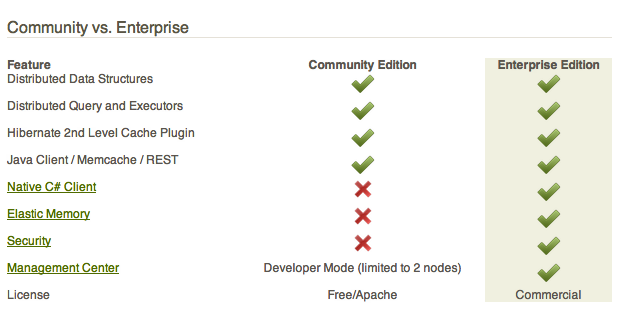
\includegraphics[scale=0.60]{hazelcast-editions.png}
For the purpose of this book we'll use the community edition. If your project relies on Maven, there is no need to install Hazelcast at all, see [link to Hazelcast and Maven]. Otherwise make sure that the Hazelcast jar is added to the classpath. Apart from this jar, there is no need to install Hazelcast.  The lack of an installation process for Hazelcast is something I really like because it saves quite a lot of time, time that can be used to solve real problems instead of environmental ones.

\section{Hazelcast and Maven}
Hazelcast is very easy to include in your Maven 3 project without needing to go through a complex installation process. Hazelcast can be found in the standard Maven repositories, so you do not need to add additional repositories to the pom. To include Hazelcast in your project, just add the following to your pom:
\begin{lstlisting}[language=xml]
<dependencies>	
    <dependency>
      <groupId>com.hazelcast</groupId>
      <artifactId>hazelcast</artifactId>
      <version>3.0</version>
   </dependency>
</dependencies>
\end{lstlisting}
That is it. Make sure that you check the Hazelcast website to make use of the most recent version. After this dependency is added, Maven will automatically downloaded the dependencies needed.

\section{Configuring Hazelcast}
Hazelcast can be configured in different ways:
\begin{enumerate}
\item programmatic configuration
\item XML configuration 
\item Spring configuration
\end{enumerate}
The programmatic configuration is the most essential one, the other mechanisms are build on top of it. In this book we'll use the xml configuration file since that is the shortest. When you are running a Maven project; just add a resources directory under src/main/ and add a file 'hazelcast.xml'. The following shows an empty configuration:
\begin{lstlisting}[language=xml]
<hazelcast xsi:schemaLocation="http://www.hazelcast.com/schema/config
                               http://www.hazelcast.com/schema/config/hazelcast-config-3.0.xsd"
           xmlns="http://www.hazelcast.com/schema/config"
           xmlns:xsi="http://www.w3.org/2001/XMLSchema-instance">
</hazelcast>
\end{lstlisting}
This example also imports an XML schema (XSD) for validation and if you are using an IDE, you probably get code completion. To reduce the size of the examples in the book, only the elements inside the <hazelcast> tags are provided. In the sources for the book you can find the full xml configuration. Another thing you might run into is the strange formatting of the java code; this is also done to reduce the size. 

In most of our examples we will rely on multicast for member discovery so that the members will join the cluster:
\begin{lstlisting}[language=xml]
<network>
   <join><multicast enabled="true"/></join>
</network>
\end{lstlisting}
See [chapter Cluster Configuration: Multicast] if multicast doesn't work or you want to know more about it. If you are using the programmatic configuration, then multicast is enabled by default.

In this book, the following approach is used to create a new Hazelcast instance:
\begin{lstlisting}[language=java]
public class Main {
    public static void main(String[] args){
        HazelcastInstance hzInstance = Hazelcast.newHazelcastInstance();
        ...
    }
}
\end{lstlisting}
The mechanism uses the following alternatives to resolve the configuration:
\begin{enumerate}
\item first checks if the 'hazelcast.config' system property is set; if it is, then the value is used as path. This is useful if you want to choose on startup of the application which hazelcast configuration file should be used. The config option can be set by adding the following to the java command: '-Dhazelcast.config=<path to the hazelcast.xml>'. The value can be a normal file path, but can also be a classpath reference if it is prefixed with 'classpath:'. 
\item else it checks if there is a 'hazelcast.xml' in the working directory.
\item after that it check if there is a 'hazelcast.xml' on the classpath. 
\item finally loads the default hazelcast configuration 'hazelcast-default.xml' that is part of the Hazelcast jar
\end{enumerate}
Also be careful to check the Hazelcast output when you are relying on an hazelcast.xml file. If it contains errors, Hazelcast will not abort the startup but will default to the 'hazelcast-default.xml'. When this happens, the system could behave completely different than you would expect.

Another option to load a HazelcastInstance, is to make use of programmatic configuration, e.g: 
\begin{lstlisting}[language=java]
public class Main {
    public static void main(String[] args){
       ExecutorConfig executorConfig = new ExecutorConfig().setPoolSize(10);
       Config config = new Config().addExecutorConfig(executorConfig);	  
       HazelcastInstance hzInstance = Hazelcast.newHazelcastInstance(config);
       ...
    }
}
\end{lstlisting}
The Hazelcast Config object has a fluent interface; meaning that the Config instance is returned when a config method on this instance is called. This makes chaining method calls very easy. The programmatic configuration is not only very useful for testing, but it also a solution for the static nature of the XML configuration. The content of the programmatic configuration can easily be created on the fly, e.g. based on database content. You could even decide to move the 'static' configuration to the hazelcast.xml, load this and then modify the dynamic parts, e.g. the network configuration.

In Hazelcast releases prior to 3.0, there was functionality for a static default HazelcastInstance, so you could say: 'Queue q = Hazelcast.getQueue("foo")'. This functionality has been removed because it lead to confusion when explicit created HazelcastInstances are combined with calls to the implicit default HazelcastInstance. So you probably want to keep a handle to the Hazelcast instance somewhere for future usage.

\section{Wildcard configuration}
The Hazelcast xml configuration can contain configuration elements for all kinds of distributed data-structures: sets, executors, maps etc. For example:
\begin{lstlisting}[language=xml]
<map name="testmap">
    <time-to-live-seconds>10</time-to-live-seconds>
</map>
\end{lstlisting}
But what if we want to create multiple map instances using the same configuration? Do we need to configure them individually? This is impossible to do if you have a dynamic number of distributed data-structures and you don't know up front how many need to be created. The solution to this problem is wildcard configuration, which is available for all data-structures. This makes it possible to use the same configuration for multiple instances. For example, we could configure the previous 'testmap' example with a 10 'time-to-live-seconds' using a wildcard configuration like this:
\begin{lstlisting}[language=xml]
<map name="testmap*">
   <time-to-live-seconds>10</time-to-live-seconds>
</map>
\end{lstlisting}
Using a single asterisk (*) character any place in the name, the same configuration can be shared by different  data-structures. The wildcard configuration can be used like this:
\begin{lstlisting}[language=java]
     Map map1 = hzInstance.getMap("testmap1");
     Map map2 = hzInstance.getMap("testmap2");
\end{lstlisting}
The maps 'testmap1' and 'testmap2' both match 'testmap*' so they will use the same configuration.

Something thing you need to watch out for are multiple configurations that match. Hazelcast will not throw an error or log a warning. Also selecting the right configuration doesn't depend on the order of definition in the configuration file and also isn't based on the best fitting match. So really make sure that your wildcard configurations are very specific. One of the ways to do it is to include the package name:
\begin{lstlisting}[language=xml]
<map name="com.foo.testmap*">
    <time-to-live-seconds>10</time-to-live-seconds>
</map>
\end{lstlisting}
A map can be loaded calling 'Map map1 = hzInstance.getMap("com.foo.testmap1")'. 

\section{Multiple Hazelcast instances}
In most cases you will have a single Hazelcast Instance per JVM. But Multiple Hazelcast Instances can run in a single JVM. This is not only useful for testing, but also for more complex setups e.g. application servers running multiple independent applications that rely on Hazelcast. Multiple Hazelcast instances can be started like this:
\begin{lstlisting}[language=java]
public class MultipleMembers {
    public static void main(String[] args){
        HazelcastInstance hzInstance1 = Hazelcast.newHazelcastInstance();
        HazelcastInstance hzInstance2 = Hazelcast.newHazelcastInstance();}}
\end{lstlisting}
When you start this multiple members, you see something like this in the output:
\begin{lstlisting}
Members [2] {
    Member [192.168.1.100]:5701 this
    Member [192.168.1.100]:5702
}
...
Members [2] {
    Member [192.168.1.100]:5701
    Member [192.168.1.100]:5702 this
}
\end{lstlisting}
As you can see there is a 2 member cluster created.

\section{Properties}
In the Hazelcast xml file properties can be included like this:
\begin{lstlisting}[language=xml]
<properties>
    <property name="property-name">property-value</property>
</properties>
\end{lstlisting}
 Apart from properties in the hazelcast.xml, they can also be passed on the commandline 'java -Dproperty-name=property-value'. One thing to watch out for; you can't override properties from the hazelcast.xml/programmatic-configuration from the command line because the latter has a lower priority. For a full listing of available properties see the 'Advanced configuration' chapter of the Hazelcast reference manual.

\section{Import}
[todo:this functionality is not yet implemented in Hazelcast 3]

\section{Variables}
[todo:this functionality is not yet implemented in Hazelcast 3]

\section{Logging}
Hazelcast supports various logging mechanisms; 'jdk', 'log4', 'sl4j' or 'none' if you don't want to have any logging. The default is 'jdk': the logging that is part of the JRE, so no additional dependencies are needed. Logging can be set by adding a property in the hazelcast.xml:
\begin{lstlisting}[language=xml]
<properties>
    <property name="hazelcast.logging.type">log4j</property>
</properties>
\end{lstlisting}
Or if you are using the programmatic configuration:
\begin{lstlisting}[language=java]
Config cfg = new Config() ;
cfg.setProperty("hazelcast.logging.type", "log4j");
\end{lstlisting}
But it can also be configured from the command line using: 'java -Dhazelcast.logging.type=log4j'. If you are going to make use of 'log4j' or 'slf4j', make sure that the correct dependencies are included. See the examples sources for more information.

If you are not satisfied with the provided logging implementations, you can always implement your own logging implementation by implementing the 'com.hazelcast.logging.LogListener'. See the Hazelcast reference manual for more information.

\section{Downloading example sources}
If you want to play around with the example sources of this book, check the following link:[todo: link to source]. 

\section{What is next?}
Hazelcast supports a lot of functionality, so we cover only the most used functionality. Some things like named HazelcastInstances have been left out. [todo: more content?]
\chapter{Distributed Primitives}
If you have programmed in Java you have probably worked with concurrency primitives like the synchronized statement (the intrinsic lock) or perhaps even the concurrency library that was introduced in Java 5 under java.util.concurrent like the Executor, Lock and AtomicReference.

This concurrency functionality is useful if you want to write a Java application that use multiple threads, but the focus is to provide is synchronization in a single JVM and not distributed over multiple JVM's. Luckily Hazelcast provides support for various distributed synchronization primitives like the Lock, IAtomicLong etc. And apart from making synchronization between different JVM's possible, they also support high availably; so if one machine fails, the primitive remains usable for other JVM's.

\section{IAtomicLong}
The IAtomicLong, formally known as the AtomicNumber, is the distributed version of the java.util.concurrent.atomic.AtomicLong, so if you have used that before, working with the IAtomicLong should feel very similar. The IAtomicLong exposes most of the operations the AtomicLong provides like get, set, getAndSet, compareAndSet and incrementAndGet, but there is of course a big difference in performance since remote calls are involved.

I'll demonstrate the IAtomicLong by creating an instance and incrementing it one million times:
\begin{lstlisting}[language=java]
public class Member {
   public static void main(String[] args) {
      HazelcastInstance hz = Hazelcast.newHazelcastInstance();
      IAtomicLong counter = hz.getAtomicLong("counter");
      for (int k = 0; k < 1000 * 1000; k++) {
         if (k % 500000 == 0) 
            System.out.println("At: "+k);
         counter.incrementAndGet();
      }
      System.out.printf("Count is %s\n", counter.get());
   }
}
\end{lstlisting}
If you start this Member, you will see this:
\begin{lstlisting}
At: 0
At: 500000
Count is 1000000
\end{lstlisting}
If you run multiple instances of this member, then the total count should be equal to one million times the number of members you have started.

If the IAtomicLong becomes a contention point in your system, there are a few ways of dealing with it, depending on your requirements. One of the options it to create a stripe (essentially an array) of IAtomicLong instances to reduce pressure. Another options is to keep changes local and only publish them to the IAtomicLong once and a while. There are a few downsides here; you could loose information if a member goes down and is that the newest value is not always immediately visible to the outside world. If you want to generate unique id's, you can have a look at the IdGenerator.

Hazelcast only provides support for the long, but you can always simulate other types:
\begin{enumerate}
\item boolean: 0 for true and 1 for false.
\item double: a 64 bit double can be encoded into 64 bits, which can be stored in a long since is also 64 bits.
\end{enumerate}
There is no support for an atomic reference, but if you need it you can build it on top of the IMap. The name of the reference could be the key and the value could be the reference value. The IMap implements the ConcurrentMap interface, so you can lift on atomic operations like replace(K key, V oldValue, V newValue). 

\section{IdGenerator}
In previous section the IAtomicLong was introduced and one of the things it can be used for is to generated unique id's within a cluster. Although it will work, it probably isn't the most scalable solution since all member will content on incrementing the value. If you are only interested in unique id's you can have a look at the com.hazelcast.core.IdGenerator.

The way the IdGenerator works is that each member claims a segment of 1 million id's to generate. This is done behind the scenes by using an IAtomicLong and claiming a segment is done by incrementing that IAtomicLong by a million. After claiming the segment, the IdGenerator can increment a local counter. Once all id's in the segment are used, it needs to claim a new segment. The consequence of this approach is that only 1 in a million times network traffic is needed; so 999.999 out of 1.000.000 the id generation can be done in memory and therefor is extremely fast. Another consequence is that this approach scales a lot better than an IAtomicLong because there is a lot less contention: 1 out of 1.000.000 instead of 1 out of 1.

So lets see the IdGenerator in action:
\begin{lstlisting}[language=java]
public class IdGeneratorMember {
   public static void main(String[] args) throws Exception{
      HazelcastInstance hz = Hazelcast.newHazelcastInstance();
      IdGenerator idGenerator = hz.getIdGenerator("id");
      for (int k = 0; k < 1000; k++){
         Thread.sleep(1000);
         System.out.printf("Id : %s\n", idGenerator.newId());
      }
   }
}
\end{lstlisting}
If you start this multiple times, you will see in the console that there will not be any duplicate id's.

Of course there are some issues you need to be aware of:
\begin{enumerate}
\item id's generated by different members will be out of order
\item if a member goes down without fully using its segment, there might be gaps.
\end{enumerate}
For id generation, in most cases, this isn't not relevant. There are alternative solutions for creating cluster wide unique id's. One of them is the java.util.UUID, although it will take up more space than a long, it doesn't rely on access to a Hazelcast cluster.

Another important issue you need to know is that if the cluster restarts, then the IdGenerator is reset and starts from 0 because the IdGenerator doesn't write to storage, e.g a database. If you need this, you can create your own IdGenerator based on the same implementation mechanism the IdGenerator uses, but you persist the updates to the IAtomicLong.

\section{ILock}
A lock is a synchronization primitive that makes it possible that only a single thread is able to access to a critical section of code; if multiple threads at the same moment would access that critical section concurrently, you would get race problems. 

Hazelcast provides a distributed lock implementation and makes it possible to create a critical section within a cluster of JVM's; so only a single thread from one of the JVM's in the cluster is allowed to acquire that lock. Other threads that want to acquire the lock, no matter if they are on the same JVM's or not, will not be able to acquire it and depending on the locking method they called, they either block or fail. The com.hazelcast.core.ILock extends the java.util.concurrent.locks.Lock interface, so using the lock is quite simple.

The following example shows how a lock can be used to solve a race problem:
\begin{lstlisting}[language=java]
public class RaceFreeMember {
   public static void main(String[] args) throws Exception {
      HazelcastInstance hz = Hazelcast.newHazelcastInstance();
      IAtomicLong number1 = hz.getAtomicLong("number1");
      IAtomicLong number2 = hz.getAtomicLong("number2");
      ILock lock = hi.getLock("lock");
      System.out.println("Started");
      for (int k = 0; k < 10000; k++) {
         if (k % 100 == 0) 
            System.out.println("at: " + k);
         lock.lock();
         try {
            if (k % 2 == 0) {
               long n1 = number1.get();
               Thread.sleep(10);
               long n2 = number2.get();
               if (n1 - n2 != 0) 
                  System.out.println("Datarace detected!");
               } else {
                    number1.incrementAndGet();
                    number2.incrementAndGet();
               }
         } finally {lock.unlock();}
      }
      System.out.println("Finished");
   }
}
\end{lstlisting}
When this code is executed; you will not see "Datarace detected!". This is because the lock provides a critical section around writing and reading of the numbers. In the example code you will also find the version with a data race.

A few things worth knowing about the Hazelcast lock and locking in general:
\begin{enumerate}
\item It is reentrant, so you can acquire it multiple times in a single thread without causing a deadlock, of course you need to release it as many times as you have acquired it, to make it available to other threads.
\item Just like with the other Lock implementations, it should always be acquired outside of a try/finally block. Else it can happen that the lock acquire failed, but an unlock is still executed. 
\item Keep locks as short as possible. If locks are kept too long, it can lead to performance problems or worse: deadlock.
\item With locks it is easy to run into deadlocks if you don't know what you are doing; so make sure that you do. Having code you don't control running inside your locks is asking for problems. Make sure you understand exactly the scope of the lock. 
\item To reduce the chance of a deadlock, the tryLock methods can be used that control the waiting period. The lock.lock() method will not block indefinitely, but will timeout with a OperationTimeoutException after 300 seconds.  
\item Locks are automatically released when a member has acquired a lock and this member goes down. This prevents threads that are waiting for a lock to wait indefinitely and needed for failover to work in a distributed system. The downside however is that if a member goes down that acquired the lock and started making changes, that other members could start to see partial changes. In these cases either the system could do some self repair or else a transaction potentially can solve the problem.
\item a lock must always be released by the same lock that acquired it, otherwise look at the ISemaphore.
\item locks are fair, so locks will be granted in the order they are requested.
\item there are no configuration options available for the lock
\item you can ask the lock if it is locked using the ILock.isLocked method.
\item a lock can be forced to unlock using the ILock.unlock method. This should be used with extreme care since it could stop a critical section from being locked. 
\end{enumerate}

[todo: lock doesn't work on name, but can be any object.. important to realize that it isn't the monitor lock of that particular 'name' you are acquiring]

\section{ICondition}
One of the new features of Hazelcast 3 is support for the ICondition which extends the java.util.concurrent.locks.Condition. Each lock can have mulitple conditions (e.g. queue full, queue empty) There is 1 difference, with the normal Java version you can create condition and depends on its reference to identify which condition you are waiting for. With Hazelcast this isn't possible since different members can't share a object reference. That is why an id is needed to identify the condition.

\begin{lstlisting}[language=java]
public class WaitingMember {
   public static void main(String[] args) throws InterruptedException {
      HazelcastInstance hz = Hazelcast.newHazelcastInstance();
      IAtomicLong counter = hz.getAtomicLong("counter");
      ILock lock = hz.getLock("lock");
      System.out.println("Starting wait");
      ICondition condition = lock.newCondition("condition");
      lock.lock();
      try {
         while (counter.get() != 1) {
            condition.await();
         }
      } finally {
         lock.unlock();
      }
      System.out.println("Wait finished");
   }
}
\end{lstlisting}

\begin{lstlisting}[language=java]
public class NotifyMember {
   public static void main(String[] args) throws InterruptedException {
      HazelcastInstance hz = Hazelcast.newHazelcastInstance();
      IAtomicLong counter = hz.getAtomicLong("counter");
      ILock lock = hz.getLock("lock");
      ICondition condition = lock.newCondition("condition");
      lock.lock();
      try {
         counter.set(1);
         condition.signalAll();
      } finally {
         lock.unlock();
      }
   }
}
\end{lstlisting}

spurious wakeups. 
signal vs signallAll

\section{ISemaphore}
The semaphore is a classic synchronization aid that can be used to control the number of threads doing a certain activity concurrently, e.g. using a resource. Conceptually each semaphore has a number of permits, where each permit represents a single thread allowed to execute that activity concurrently. As soon as a thread want to start with the activity, it takes a permit (or waits until one becomes available) and once finished with the activity, the permit is returned.

If you initialize the semaphore with a single permit, it looks a lot like a lock. One of the big difference is that the Semaphore has no concept of ownership. So with a lock the thread that acquired the lock must release it, but with a semaphore any thread can release an acquired permit. Another difference is that an exclusive lock only has 1 permit and a semaphore can have more than 1.

Hazelcast provides a distributed version of the java.util.concurrent.Semaphore named the com.hazelcast.core.ISemaphore. When a permit is acquired on the ISemaphore the following can happen:
\begin{enumerate}
\item a permit is available. The number of permits in the semaphore is decreased by one and the calling thread can continue. 
\item no permit is available. The calling thread will block until a permit comes available, a timeout happens, the thread is interrupted or when the semaphore is destroyed an InstanceDestroyedException will be thrown.
\end{enumerate}
I'll explain the semaphore with an example. To simulate a shared resource we have an IAtomicLong initialized with the value 0. This resource is going to used 1000 times, When a thread starts to use that resource it increments it and once completed it decrements it.
\begin{lstlisting}[language=java]
public class SemaphoreMember {
   public static void main(String[] args)throws Exception{
      HazelcastInstance hz = Hazelcast.newHazelcastInstance();
      ISemaphore semaphore = hz.getSemaphore("semaphore");
      IAtomicLong resource = hz.getAtomicLong("resource");
      for(int k=0;k<1000;k++){
         System.out.println("At iteration: "+k +
            ", Active Threads: " + resource.get());
         semaphore.acquire();
         try{
            resource.incrementAndGet();
            Thread.sleep(1000);
            resource.decrementAndGet();
         }finally{semaphore.release();}
      }
      System.out.println("Finished");
   }
}
\end{lstlisting}
We want to limit the concurrent access to the resource by allowing for at most 3 thread. This can be done by configuring the initial-permits for the semaphore in the Hazelcast config file:
\begin{lstlisting}[language=xml]
<semaphore name="semaphore">
   <initial-permits>3</initial-permits>
</semaphore>
\end{lstlisting}
When you start the SemaphoreMember 5 times you will see output like this:
\begin{lstlisting}
At iteration: 0, Active Threads: 1
At iteration: 1, Active Threads: 2
At iteration: 2, Active Threads: 3
At iteration: 3, Active Threads: 3
At iteration: 4, Active Threads: 3
\end{lstlisting}
As you can see the maximum number of concurrent threads using that resource always is equal or smaller than 3. As an experiment you can remove the semaphore acquire/release statements and see for yourself that there is no longer control on the number of concurrent usages of the resources.

A few things worth knowing about the ISemaphore:
\begin{enumerate}
\item fairness: the Semaphore acquire methods are fair and this is not configurable. So under contention, the longest waiting thread for a permit will acquire it before all other threads. This is done to prevent starvation, at the expense of reduced throughput.
\item attach permits: one of the features added to the ISemaphore to make it more reliable in a distributed environment where failover is important, is the addition of attached permits. Normally when a permit is acquired, and the member that acquired the permit goes down, the permit is not released. The consequence is that the permit is lost and the maximum number of concurrent threads for a specific activity is reduced. It can even lead to a deadlock situation when the number of available permits reaches 0. With the attached permits, the permit is attached to a member, and when it goes down, the permit is automatically released (similar as with the Hazelcast Lock).
\item the acquire() method doesn't timeout, unlike the Hazelcast Lock.lock() method. To prevent running into a deadlock, using one of timed acquire methods is a good solution.
\end{enumerate}

[TODO: Semaphore factory.]

\section{ICountDownLatch}
The java.util.concurrent.CountDownLatch was introduced in Java 1.5 and is a synchronization aid that makes it possible for threads to wait until a set of operations, being performed by one or more threads to complete. Very simplistically; a CountDownLatch could be seen as a gate containing a counter. Behind this gate, threads can wait till the counter reaches 0. In my experience CountDownLatches often are used when you have some kind of processing operation, and one or more threads need to wait till this operation completes so they can execute their logic. Hazelcast also contains a CountDownLatch; the org.hazelcast.core.ICountDownLatch.

To explain the ICountDownLatch, image there is a leader process that is executing some action and eventually completes. And imagine that there are one or more follower processes that need to do something after the leader has completed. We can implement the behavior of the Leader:
\begin{lstlisting}[language=java]
public class Leader{
   public static void main(String[] args)throws Exception{
      HazelcastInstance hz = Hazelcast.newHazelcastInstance();
      ICountDownLatch latch = hz.getCountDownLatch("latch");      
      System.out.println("Starting");
      latch.trySetCount(1); 
      Thread.sleep(5000);
      latch.countDown();
      System.out.println("Leader finished");
      latch.destroy();
   }
}
\end{lstlisting}
The Leader retrieves the CountDownLatch, calls trySetCount on it which makes him owner of that latch, does some waiting and then calls countdown; which notifies are listeners for that latch. Currently we ignore the boolean return value of trySetCount since there will only be a single Leader, but in practice you probably want deal with the return value. Although there will only be a single owner of the Latch, the countDown method can be called by other threads/processes.

The next part is the Follower:
\begin{lstlisting}[language=java]
public class Follower {
   public static void main(String[] args) throws Exception {
      HazelcastInstance hz = Hazelcast.newHazelcastInstance();
      ICountDownLatch latch = hz.getCountDownLatch("latch");
      System.out.println("Waiting");
      boolean success = latch.await(10, TimeUnit.SECONDS);
      System.out.println("Complete:"+success);
  }
}
\end{lstlisting}
As you can see we first retrieve the ICountDownLatch and then call await on it so the thread listens for the ICountDownLatch to reach 0. In practice it can happen than a process that should have called the ICountDownLatch.countDown method, fails and therefor the ICountDownLatch will never reach 0. To force you to deal with this situation, there is no await method without a timeout to prevent waiting indefinitely. 

If we first start a leader and then one or more followers, the followers will wait till the leader completes. It is important that the leader is started first, else the followers will immediately complete since the latch already is 0. The example show a ICountDownLatch with only a single step. But if a process has n steps, initialize the CountdownLatch with n instead of 1 and for each completed step call the countDown method.

One thing to watch out for is that a ICountDownLatch waiter can be notified prematurely. In a distributed environment the leader could go down before it has reached zero and this would result in the waiters to wait till the end of time. This behavior is undesirable, so Hazelcast will automatically notify all listeners if the ICountDownLatch owner gets disconnected. So it can be that listeners are notified before all steps of a certain process are completed. To deal with this situation the current state of the process needs to be verified and appropriate actions need to be undertaken. e.g. restart all operations, continue with the first failed operation, or throw an exception.

Although the ICountdownLatch is a very useful synchronization aid, it probably isn't one you will use on a daily basis. Unlike Java's implementation, Hazelcast's ICountDownLatch count can be re-set after a countdown has finished but not during an active count. 

\section{Good to know}

\emph{Not interruptible:}

\section{What is next?}
In this chapter we looked at various synchronization primitives that are supported by Hazelcast. If for whatever reason you need a different one you can try to build it on top of existing ones, or create a custom one using the Hazelcast SPI. One of the things I would like to see added the ability to control the partition the primitive is living on since this would improve locality of reference. 

\chapter{Distributed Collections}
Hazelcast provides a set of collections that implement interfaces from the Java collection framework and therefor make it easy to integration distributed collections in your system without too many code changes. A distributed collection can not only be called concurrently from the same JVM, it also can be called concurrently by different JVM's. Another advantage is that the distributed collections provide high availability, so if a member hosting the collection fail, another member will take over.

\section{IQueue}
A BlockingQueue is one of the work horses for concurrent system because it allows producers and consumers of messages, which can be POJO's, to work different speeds. The Hazelcast com.hazelcast.core.IQueue, which extends the java.util.concurrent.BlockingQueue, not only allows threads from the same JVM to interact with that queue, but since the queue is distributed, it also allows different JVM's to interact it. So you can add items in one JVM and remove them in another.

As an example we'll create a producer/consumer implementation that is connected by a distributed queue. The producer is going to put a total of 100 Integers on the queue with a rate of 1 message/second.
\begin{lstlisting}[language=java]
public class ProducerMember {
    public static void main(String[] args) throws Exception {
        HazelcastInstance hz = Hazelcast.newHazelcastInstance();
        IQueue<Integer> queue = hz.getQueue("queue");
        for (int k = 1; k < 100; k++) {
            queue.put(k);
            System.out.println("Producing: " + k);
            Thread.sleep(1000);
        }
        queue.put(-1);
        System.out.println("Producer Finished!");
    }
}
\end{lstlisting}
To make sure that the consumers are going to terminate when the producer is finished, the producer will put a -1 on the queue to indicate that it is ready. 

The consumer will take the message from the queue, print it and waits 5 seconds before consuming the next message and stops when it receives the -1, also called a poison pill:
\begin{lstlisting}[language=java]
public class ConsumerMember {
    public static void main(String[] args) throws Exception {
        HazelcastInstance hz = Hazelcast.newHazelcastInstance();
        IQueue<Integer> queue = hz.getQueue("queue");
        while (true){
            int item = queue.take();
            System.out.println("Consumed: " + item);
            if(item == -1){
                queue.put(-1);
                break;
            }     
            Thread.sleep(5000);
        }
        System.out.println("Consumer Finished!");
    }
}
\end{lstlisting}
If you take a closer look at the consumer, you see that when the consumer receives the poison pill, it puts the poison pill back on the queue before it ends the loop. This is done to make sure that all consumer will also receive the poison pill, and not only the one that received it first.

When you start a single producer, you will see the following output:
\begin{lstlisting}
Produced 1
Produced 2
....
\end{lstlisting}
When you start a single consumer, you will see the following output:
\begin{lstlisting}
Consumed 1
Consumed 2
....
\end{lstlisting}
As you can see, the items produced on the queue by the producer are being consumed from that same queue by the consumer. 

Because messages are produced 5 times faster than they are consumed, with a single member the queue will keep growing. To improve throughput, you can start more consumers. If we start another one, we'll see each consumer takes care of half the messages. Consumer 1:
\begin{lstlisting}
Consumed 20
Consumed 22
....
\end{lstlisting}
Consumer 2:
\begin{lstlisting}
Consumed 21
Consumed 23
....
\end{lstlisting}
When you kill one of the consumers, the remaining consumer will process all elements again:
\begin{lstlisting}
Consumed 40  
Consumed 42 
....
\end{lstlisting}
One thing to take care of that if there are many producers/consumers interacting with the queue, is that there will be a lot of contention and eventually the queue will become the bottleneck. One way of solving this problem is to introduce a stripe (essentially a list) of queues. But if you do, the ordering of messages send to different queues will not be guaranteed anymore. In a lot of cases a strict ordering isn't required and a stripe can be a simple solution to improve scalability.

\emph{Important}: Realize that although the Hazelcast distributed queue preserves ordering of the messages (so the messages are taken from the queue in the same order they were put on the queue), if there are multiple consumers, the processing order is not guaranteed because the queue will not provide any ordering guarantees on messages after they are taken.

\subsection{Capacity}
In the previous example we showed a basic producer/consumer solution based on a distributed queue. Because the production of messages is separated from the consumption of messages, the speed of production is not influenced by the speed of consumption. If producing messages goes quicker than the consumption, then the queue will increase in size. If there is no bound on the capacity of the queue, then machines can run out of memory and you will get an OutOfMemoryError. 

With the traditional BlockingQueue implementations, like the LinkedBlockingQueue, a capacity can be set. When this is set and the maximum capacity is reached, placement of new items either fail or block, depending on type of the put operation. This prevents the queue from growing beyond a healthy capacity and the JVM from failing.

The Hazelcast queue also provided capacity control, but instead of having a fixed capacity for the whole cluster, Hazelcast provides a scalable capacity by setting the queue capacity per member using the queue property max-size. So if the capacity per member is 1000 and there are 5 members's, the total capacity is 5000. Therefor the capacity depends on the size of the cluster. To give our queue a capacity of 10 per member, we set the max-size:
\begin{lstlisting}
<network>
    <join><multicast enabled="true"/></join>
</network>
<queue name="queue">
    <max-size>10</max-size>
</queue>
\end{lstlisting}
When we start a single producer, we'll see that 10 items are produced and then the producer blocks. If we then start a single consumer, we'll immediately see that the producer will continue since the total capacity for the queue has doubled to 20 (2 JVM's times 10 items per JVM). 

But since the producer produces 5 times as fast as the consumer, the queue will reach its maximum capacity again quickly and it will block. We can can increase the capacity of the cluster by starting new consumers (both processing and the storage capacity increase) or just empty members (the storage capacity increases).

\subsection{Backups}
By default Hazelcast will make sure that there is one synchronous backup for the queue; so if the member hosting that queue fails, the backups on another member will be used so no entries is lost.

Backups can be controlled using the async-backup-count which defaults to 0 and backup-count which defaults to 1. If you want increased high availability you could either increase the backup-count or the async-backup-count. If you want to have improved performance you could remove the synchronous backup and replace it with a asynchronous backup, so there is a small chance of failure, or you disable backups if entries are allowed to be lost. 

\subsection{QueueStore}
By default Hazelcast data-structures like the IQueue are not persistent:
\begin{enumerate}
 \item if the cluster starts, the queues will not be populated by themselves.
 \item changes in the queue will not be made persistent, so if the cluster fails then entries will be lost.
\end{enumerate}
In some cases this behavior is not desirable and luckily Hazelcast provide a mechanism for queue durability using the QueueStore which can read and write to a database for example. In Hazelcast 2 the Queue was implemented on top of the Hazelcast Map, so in theory you could make the queue persistent by configuring the MapStore of the backing map. In Hazelcast 3, the Queue is not implemented on top of a map anymore but luckily exposes a QueueStore directly.

[todo: example]

\section{IList}
A List is a collection where every element only occurs ones and where the order of the element doesn't matter. The Hazelcast com.hazelcast.core.IList implements the java.util.List. We'll demonstrate the IList by adding items to a list on one member and on another member we print the elements from that list:
\begin{lstlisting}[language=java]
public class WriteMember {
   public static void main(String[] args) {
      HazelcastInstance hz = Hazelcast.newHazelcastInstance();
      IList<String> list = hz.getList("list");
      list.add("Tokyo");
      list.add("Paris");
      list.add("New York");
      System.out.println("Putting finished!");
   }
}
public class ReadMember {
   public static void main(String[] args) {
      HazelcastInstance hz = Hazelcast.newHazelcastInstance();
      IList<String> list = hz.getList("list");
      for (String s : list) 
         System.out.println(s);
      System.out.println("Reading finished!");
   }
}
\end{lstlisting}
If you first run the WriteMember and after it has completed, start the ReadMember then the ReadMember will output the following:
\begin{lstlisting}
Tokyo
Paris
New York
Reading finished!
\end{lstlisting}
As you can see, the data written to the List by the WriteMember is visible in the ReadMember and you also can see that the order is maintained. The List interface has various methods like the sublist that returns collections, it is important to understand that the returned collections are snapshots and are not backed up the by list. See [reference 'weak consistency' iterators at end of chapter]

\section{ISet}
A Set is a collection where every element only occurs once and where the order of the elements doesn't matter. The Hazelcast com.hazelcast.core.ISet implements the java.util.Set. I'll demonstrate the set by adding items in a Set on one member, and on another member we are going to print all the elements from that Set:
\begin{lstlisting}[language=java]
public class WriteMember {
   public static void main(String[] args) {
      HazelcastInstance hz = Hazelcast.newHazelcastInstance();
      ISet<String> set = hz.getSet("set");
      set.add("Tokyo");
      set.add("Paris");
      set.add("New York");
      System.out.println("Putting finished");
   }
}
public class ReadMember {
   public static void main(String[] args) {
      HazelcastInstance hz = Hazelcast.newHazelcastInstance();
      ISet<String> set = hz.getSet("set");
      for(String s: set) 
         System.out.println(s);
      System.out.println("Reading finished!");
   }
}
\end{lstlisting}
If you first start the WriteMember and waiting for completion, you start the ReadMember; it will output the following:
\begin{lstlisting}
Paris
Tokyo
New York
Reading finished!	
\end{lstlisting}
As you can see, the data added by the WriteMember is visible in the ReadMember. As you also can see, the order is not maintained since order is not defined by the Set.

Just as with normal HashSet, the hash and equals of the object are used and not the equals/hash of the byte array version of that object. This is different behavior compared to the map; see [reference to equals/hash section in the map]

In Hazelcast the ISet (and same goes for the IList) is implemented as a collection within the MultiMap, where the id of the set is the key in the multimap and the value is the collection. This means that the ISet is not partitioned, so you can't scale beyond the capacity of a single machine and you can't control the partition where data from a set is going to be stored. If you want to have a distributed set that behaves more like the distributed map, one simple option is to implement a set based on a map, where the value can be some bogus value. It isn't possible to rely on the Map.keySet for returning a usable distributed set since it will return a non distributed snapshot of the keys.

\section{Collection ItemListener}
The IList, ISet and IQueue interfaces extend the com.hazelcast.core.ICollection interface. The nice thing is that Hazelcast enriches the existing collections api with the ability to listen to changes in the collections using the com.hazelcast.core.ItemListener. The ItemListener receives the ItemEvent which not only potentially contains the item, but also the member where the changed happened and the type of event (add or remove).

The following example shows an ItemListener that listens to all changes made in an IQueue:
\begin{lstlisting}[language=java]
public class ItemListenerMember {
   public static void main(String[] args) throws Exception {
      HazelcastInstance hz = Hazelcast.newHazelcastInstance();
      ICollection<String> q = hz.getQueue("queue");
      q.addItemListener(new ItemListenerImpl<String>(), true);
      System.out.println("ItemListener started");
   }
   private static class ItemListenerImpl<E> 
      implements ItemListener<E> {
      public void itemAdded(ItemEvent<E> e) {
         System.out.println("Item added:" + e.getItem());
      }
      public void itemRemoved(ItemEvent<E> e) {
         System.out.println("Item removed:" + e.getItem());
      }
   }
}
\end{lstlisting}
We registered the ItemListenerImpl with the addItemListener method using the value 'true'. This is done to make sure that our ItemListenerImpl will get the value that has been added/removed. The reason this configuration option is available, is that in some cases you only want to be notified that a change happened, but you're not interested in the actual change and don't want to pay for sending the value over the line.

To see that the ItemListener really is working, we'll create a member that makes a change in the queue:
\begin{lstlisting}[language=java]
public class CollectionChangeMember{
   public static void main(String[] args) throws Exception {
      HazelcastInstance hz = Hazelcast.newHazelcastInstance();
      BlockingQueue<String> q = hz.getQueue("queue");
      q.put("foo");
      q.put("bar");
      q.take();
      q.take();
   }
}
\end{lstlisting}
First start up the ItemListenerMember and wait till it displays "ItemListener started". After that start the CollectionChangeMember and you will see the following output in the ItemListenerMember:
\begin{lstlisting}
item added:foo
item added:bar
item removed:foo
item removed:bar
\end{lstlisting}
ItemListeners are useful if you need to react upon changes in collections. But realize that listeners are executed asynchronously, so it could be that at the time your listener runs,  the collection has changed again. 

\emph{Ordering} All events are ordered, which means that listeners will receive and process the events in the order they are actually occurred. 

\section{Good to know}

\emph{Iterator stability:} Iterators on collections are weakly consistent; meaning that when a collection changes while creating the iterator, you could encounter duplicates or miss element. Changes on that iterator will not result in changes on the collection. An iterator doesn't need to reflect the actual state and will not throw a ConcurrentModifcationException. 

\emph{Not Durable:} In Hazelcast 2 the IQueue/IList/ISet were build on top of the Hazelcast distributed map and by accessing that map you could influence the collections their behavior including storage. This isn't possible anymore in Hazelcast 3. The IQueue now has its own QueueStore mechanism, but the List/Set have not. Perhaps this will be added in a later release.

\emph{Replication:} The replication for IList and ISet can't be configured and will automatically have 1 synchronous backup and 1 asynchronous backups. Perhaps in the future this is going to be configurable.

\emph{Destruction:} IQueue/ISet/IList instances immediately are 'destroyed' when they are empty and will not take up space. Listeners will remain registered, unless that collection is destroyed explicitly. Once an item is added to implicit destroyed collection, the collection will automatically be recreated.

\emph{Not partitioned:}  The IList/ISet are implemented as a collection in a MultiMap. and therefor are not partitioned; so their size can't grow beyond the capacity of a single JVM. This is a big difference compared to Hazelcast 2.x where they were partitioned. This limitation needs to be taken into consideration when you are designing a distributed system. A few ways to solve this issue are to use a stripe of collections or to build your collection on top of the IMap. Another more flexible but probably more time consuming alternative is to write the collection on top of the new SPI functionality [reference to SPI chapter]

\section{What is next?}
The API's shown in these examples is only a subsection of what Hazelcast collections provides. todo: more text.
\chapter{Distributed Map}
In this chapter, you'll learn how to use one of the most versatile data structures in Hazelcast; the com.hazelcast.core.IMap. The IMap extends the java.util.concurrent.ConcurrentMap interface, and therefor it also extends the java.util.Map but its implementation is designed to be used in a distributed environment. So changes made in one member are visible in another and when a member fails, backups will be restored an the cluster can continue as if nothing happened.

Internally Hazelcast divides the map in partitions, by default 271 and can be changed with the 'hazelcast.map.partition.count' property, and distributes the partitions evenly among the members in the cluster. The partition is determined based on the key; each key belongs to a single partition. 

Scaling up is simple; just add more members and they will take their share of the load. The oldest member decides which partitions need to be moved to the new members and chooses partitions that contain the least amount of data to reduce network traffic. Hazelcast doesn't do any runtime rebalancing of partitions e.g. based on partition size or usage. 

Scaling down also is simple; just shutdown the HazelcastInstances to release their share of the load. The partitions will automatically be reassigned to other members. Of course a hard kill of the JVM is possible, but then you run a risk of loosing something if you have not configured the backup mechanism correctly; see [reference to backup section]

The commercial offering of Hazelcast includes Elastic Memory where the map entries are not stored in the Java Heap to drastically reduce gc times. On Youtube there is demo: http://www.youtube.com/watch?v=TOhbhKqJpvw where 4 Terabyte of data from 1 billion entries is stored on 100 Amazon EC2 instances, supporting to 1.3 million of operations/second.

\section{Reading/Writing}
The Hazelcast Map implements the ConcurrentMap/Map interface, so reading/writing key/values is very simple since you can use familiar methods like get/put etc. 

To demonstrate this basic behavior a distributed is created in a member and some entries are written to this map. In another member these entries are going to be read and printed:
\begin{lstlisting}[language=java]
public class FillMapMember {
    public static void main(String[] args) {
        HazelcastInstance hzInstance = Hazelcast.newHazelcastInstance();
        Map<String, String> employees = hzInstance.getMap("employees");
        employees.put("1", "Tokyo");
        employees.put("2", "Paris");
        employees.put("3", "New York");
    }
}
\end{lstlisting}
As you can see the Map is retrieved using the hzInstance.getMap(mapName) and then some entries are stored in that map. Reading the entries can be done like this:
\begin{lstlisting}[language=java]
public class PrintAllMember {
    public static void main(String[] args) {
        HazelcastInstance hzInstance = Hazelcast.newHazelcastInstance();
        Map<String, String> employees = hzInstance.getMap("employees");
        for(Map.Entry<String,String> entry : employees.entrySet())
            System.out.println(entry.getKey()+" "+entry.getValue());
    }
}
\end{lstlisting}
If the FillMapMember is runs before the PrintAllMember, we'll get output like this:
\begin{lstlisting}
3 New York
1 Tokyo
2 Paris
\end{lstlisting}
As you can see, the map updates from the FillMapMember are visible in the PrintAllMember.

Internally Hazelcast will serialize the key/values (see chapter Serialization) to byte arrays and store this in the underlying storage mechanism. This means changes made to a key/value after they are stored in the map, will not reflect on the stored state. Therefor the following idiom is broken:
\begin{lstlisting}[language=java]
Employee e  = employees.get(123);
e.setFired(true);
\end{lstlisting}
If you want this change to be stored in the map, you need to put the updated value back:
\begin{lstlisting}[language=java]
Employee e  = employees.get(123);
e.setFired(true);
employees.put(123,e);
\end{lstlisting}

\subsection*{record type}
Apart from writing the update back to the map, there is another very important setting called 'cache-value'. When the value is read from a map, the value is deserialized since the map contains the serialized value. The problem is that this can lead to a lot of deserialization overhead if the value is read frequently. To reduce this overhead, if the member owns the key, the value instance can be cached. So multiple requests for some key that is owned by that member, will result in the same instance being returned instead of a copy. 

This works very fine if the value is an immutable object, but if the value is a mutable object, it can lead to unexpected sharing. This can cause all kinds of problems like race problems and JMM problems. By default 'cache-value' is set to true, so if you store mutable objects in your map, you need to explicitly set 'cache-value' to false, e.g:
\begin{lstlisting}[language=xml]
<map name="employees">
    <cache-value>false</cache-value>
</map>
\end{lstlisting}
This only need to be done with the map, the other data structures that are build on top of the map like the Queue do not cache the value. The cashed value is stored directly in local map entry, so the size of the cache will always be equal or smaller than the number of local map entries. This means that there will be extra memory usage, but it will not grow uncontrollable.

One thing to watch out for is that when you put an item in a cache-value enabled map, it will not return that instance on a subsequent read, but it will return a copy (due to deserialization). This copy will be cached, not the original instance.

RecordType.DATA: Hazelcast will store values in the object class DataRecord which stores the value in its serialized form.

RecordType.OBJECT: Hazelcast will store values in the class ObjectRecord which stores the value in its de-serialized object form.

RecordType.CACHED: Hazelcast will store values in the class CachedDataRecord which stores the value in its de-serialized object form but also caches the deserialized object.

The default record type is DATA. You should consider using OBJECT if majority of your hazelcast usage is composed of queries and entry processors.

If you have been using Hazelcast 2.x you might remember the cache-value property. This is the Hazelcast 3 version of it.

\section{Hashcode and equals}
In most cases you probably will make use of some basic type like a Long, Integer or String as key. But in some cases you will need to create custom keys. But to do it correctly in Hazelcast, you need to understand how this mechanism works because it works differently compared to traditional map implementations. When you store a key/value in a Hazelcast map, instead of storing the Object, the object are serialized to byte arrays and these are stored. To use the hash/equals in Hazelcast you need to know the following rules:
\begin{enumerate}
\item for keys: the hash/equals is determined based on the content of the byte array, so equal keys need to result in equal byte arrays.
\item for values: the hash/equals is determined based on the deserialized object, and not the hash/equals of the byte array content. 
\end{enumerate}
As you can see the difference is subtile, but it is crucial to understand.

Below is an example of a key implementation that is valid for a map implementation like the HashMap, but invalid when it is used in a Hazelcast map:
\begin{lstlisting}[language=java]
public final class BrokenKey implements Serializable {
    private final String significant;
    private final String insignificant;
    public BrokenKey(String significant, String insignificant) {
        this.significant = significant;
        this.insignificant = insignificant;
    }
    public boolean equals(Object o) {
        if (this == o) return true;
        if (!(o instanceof BrokenKey)) return false;
        BrokenKey that = (BrokenKey) o;
        return that.significant.equals(this.significant);
    }
    public int hashCode() {
       return significant.hashCode();
   }
}
\end{lstlisting}
This BrokenKey has 2 fields; the significant field is used in the hash/equals implementation and the insignificant field is not. If we would make 2 keys:
\begin{lstlisting}
BrokenKey key1 = new BrokenKey("a","b");
BrokenKey key2 = new BrokenKey("a","c");
\end{lstlisting} 
then 'key1.equals(key2)' and 'key1.hashCode()==key2.hashCode()'. So if a value would be put with key1, it can be retrieved using key2. But because the byte array of key1 (which will contains 'a' and 'b') is different than the byte array of key2 (which will contain 'a' and 'c'), the hash code and equals be different. 

[TODO:Note that the distributed Set and List stores its entries as the keys in a distributed Map. So the notes above apply to the objects you store in Set and List.]

\section{Distributed Queries}
Imagine that we have a Hazelcast IMap where the key is some id and the value is Person object and we want to retrieve all persons with a given name. We could create the following very naive implementation:
\begin{lstlisting}[language=java]
   public Set<Person> getWithNameNaive(String name){
        Set<Person> result = new HashSet<Person>();
        for(Person person: personMap.values())
            if(person.name.equals(name))
                result.add(person);
        return result;
    }
\end{lstlisting}
This is what you probably would write if the map would be an ordinary map. But when the map is distributed map, there are some performance and scalability problems with this approach:
\begin{enumerate}
\item It is not parallelizable. One member will iterate over all persons instead of spreading the load over multiple members. Because the search isn't parallelizable, the system can't scale; you can add more members to the cluster to increase performance.
\item It is inefficient because all persons need to be pulled over the line before being deserialized into the memory of the executing member. So there is a huge amount of network traffic because all data go over the line.
\end{enumerate}

Luckily Hazelcast solves these problems by supporting predicates that are executed on top of a fork/join mechanism:
\begin{enumerate}
\item when the predicate is requested to be evaluated by the caller, it is forked to each member in the cluster
\item each member will filter all local map entries using the predicate. Before a predicate evaluates a map entry, the key/value of that entry are deserialized and passed to the predicate. 
\item the caller joins on the completion of all members and merges the results into a single set
\end{enumerate}
The fork/join approach is highly scalable because it parallelizable. By adding additional cluster members, the number of partitions per member is reduced and therefor the time a member needs to iterate over all its data, is reduced as well. Also the local filtering is parallelizable because a pool of 'partition threads' will evaluate segments of elements concurrently. And last but not least, the amount of network traffic is reduced drastically, since only filtered data is send instead of all data.

Hazelcast provides 2 API's for distributed queries:
\begin{enumerate}
\item Criteria API
\item Distributed SQL Query
\end{enumerate}

\subsection*{Criteria API}
To implement the Person search using the criteria API, it could be as simple as this:
\begin{lstlisting}[language=java]
    public Set<Person> getWithName(String name) {
        Expression getNameExpression = Predicates.get("name");
        Predicate predicate = Predicates.equal(getNameExpression, name);
        return (Set<Person>) personMap.values(predicate);
    }
\end{lstlisting}
First we need to get the name of the Person. This is done by the 'get' expression. Then we need to create an equal predicate that has as input the expression that gets the name and the other input is the name we are looking for. After we have created the predicate, we apply it to the personMap by calling the 'IMap.values(Predicate)' method which takes care of sending it to all members in the cluster, evaluating it, and merging the result. The Predicate is not limited to values only. It can also apply be applied to the keySet, the entrySet and the localKeySet of the IMap. 

\subsubsection*{Get expression}
In the previous example we already saw the get expression in action where it gets the name of the person object. When it is evaluated, it first tries to lookup an accessor method, so in case of 'name', the accessor methods it will try are 'isName()' and 'getName()'. If one found, it is called and the evaluation has completed. Of course an accessor method doesn't need to return a field, it could also be a synthetic accessor where some value is determined on the fly. If no accessor is found, a field with the given name is looked up. If that exists, it is returned and otherwise a RuntimeException is thrown. Hazelcast doesn't care about the accessibility of a field or an accessor method, so you are not forced to make them public.

In some cases you need to traverse over an object structure, e.g. we want the street of the address the person lives at. With the get expression this can be done like this: 'address.street'. This expression is evaluated from left to right and there is no limit on the number of steps involved. Also accessor methods can be used here. Another thing important to know is how the get expression deals with null, especially with object traversal. As soon null is found, null is returned instead of a NullPointerException being thrown. So if address would be null, the evaluation of the get expression 'address.street' will return null.

If you find the get expression too limited, you can create your own expression by extending the com.hazelcast.query.Expression interface:
\begin{lstlisting}[language=java]
public interface Expression<T> extends Serializable {
    T getValue(Object obj);
}
\end{lstlisting}

\subsubsection*{And, Or and Not predicates}
Predicates can be joined using the 'and' and 'or' predicate:
\begin{lstlisting}[language=java]
   ...
   public Set<Person> getWithNameAndAge(String name, int age) {
      Predicate namePredicate = equal(get("name"), name);
      Predicate agePredicate = equal(get("age"), age);
      Predicate predicate = and(namePredicate, agePredicate);
      return (Set<Person>) personMap.values(predicate);
   }
   public Set<Person> getWithNameOrAge(String name, int age) {
       Predicate namePredicate = equal(get("name"), name);
       Predicate agePredicate = equal(get("age"), age);
       Predicate Person = or(namePredicate, agePredicate);
       return (Set<Person>) personMap.values(predicate);
   }
\end{lstlisting}
And of course we can't forget the 'not' predicate:
\begin{lstlisting}[language=java]
    public Set<Person> getNotWithName(String name) {
        Predicate namePredicate = equal(get("name"), name);
        Predicate predicate = not(namePredicate);
        return (Set<Person>) personMap.values(predicate);
    }
\end{lstlisting}

\subsubsection*{Other predicates}
In the Predicates class you can find a whole collections of useful predicates:
\begin{enumerate}
\item notEqual: checks if the result of an expression is not equal to a certain value.
\item instanceOf: checks if the result of an expression has a certain type
\item like: checks if the result of an expression matches some string pattern. \% (percentage sign) is placeholder for many characters, \_ (underscore) is placeholder for only one character.
\item greaterThan: checks if the result of an expression is greater than a certain value.
\item greaterEqual: checks if the result of an expression is greater or equal than a certain value.
\item lessThan: checks if the result of an expression is less than a certain value
\item lessEqual: checks if the result of an expression is than than or equal to a certain value.
\item between: checks if the result of an expression is between 2 values (this is inclusive).
\item in: checks if the result of an expression is an element of a certain collection.
\item isNot: checks if the result of an expression is false.
\item regular expression: checks if the result of an expression matches some regular expression. Although there is no static convenience function for it on Predicates, the Predicates.RegexPredicate is publicly available.
\end{enumerate}
If the predicates provided by Hazelcast are not enough, you can always write your own predicate by implementing the Predicate interface:
\begin{lstlisting}[language=java]
public interface Predicate<K, V> extends Serializable {
    boolean apply(MapEntry<K, V> mapEntry);
}
\end{lstlisting}
The MapEntry not only contains the key/value, but also contains all kinds of metadata like the time it was created/expires/last-accessed etc. 

\subsubsection*{PredicateBuilder}
The syntax we used so far to create Predicates is clear but can be simplified by making use of the PredicateBuilder. It provides a fluent interface that can make building predicates simpler. But underwater the same functionality is being used. Here is an example where a predicate is build that selects all persons with a certain name and age using this PredicateBuilder:
\begin{lstlisting}[language=java]
    public Set<Person> getWithNameAndAgeSimplified(String name, int age) {
        EntryObject e = new PredicateBuilder().getEntryObject();
        Predicate predicate = e.get("name").equal(name).and(e.get("age").equal(age));
        return (Set<Person>) personMap.values(predicate);
    }
\end{lstlisting}
As you can see, it can simplify things, especially if you have complex predicates. But it is a matter of taste which approach you prefer.

\subsection*{Distributed SQL Query}
In the previous section the Criteria API was explained where expression/predicate objects are manually created. The pain can be reduced a bit by making use of the PredicateBuilder, but it still isn't perfect. That is why a DSL was added: the Distributed SQL Query, that is based on a SQL like language. But underwater the Criteria API is used. 

The 'get with name' function we already implemented using the Criteria API, can be implementing using the Distributed SQL Query like this:
\begin{lstlisting}
public Set<Person> getWithName(String name){
    Predicate predicate = new SqlPredicate(String.format("name = %s",name));
    return (Set<Person>) personMap.values(predicate);
}
\end{lstlisting}
As you can see, the SqlPredicate is a Predicate itself and therefor can be combined with the Criteria API. The language itself isn't case sensitive, but 'columns' used in the query are. Underneath you can see an overview of the DSL:
\begin{enumerate}
	\item logical operators
	\begin{lstlisting}
man and age>30
man=false or age = 45 or name = 'Joe'
man and (age >20 OR age < 30)
not man
	\end{lstlisting}

	\item relational operators
	\begin{lstlisting}
age <= 30
name ="Joe"
age != 30
	\end{lstlisting}

	\item between
	\begin{lstlisting}
age between 20 and 33
age not between 30 and 40
	\end{lstlisting}

	\item like
	\begin{lstlisting}
name like 'Jo%' (true for 'Joe', 'Josh', 'Joseph' etc.)
name like 'Jo_' (true for 'Joe'; false for 'Josh')
name not like 'Jo_' (true for 'Josh'; false for 'Joe')
name like 'J_s%' (true for 'Josh', 'Joseph'; false 'John', 'Joe')
	\end{lstlisting}
	\item in
	\begin{lstlisting}
age in (20, 30, 40)
age not in (60, 70)
	\end{lstlisting}
\end{enumerate}

\section{Indices}
To speed up queries, just like in databases, the Hazelcast map supports indices. Using an index prevents from iterating over all values (in database terms this is called a full table scan), but directly jump to the interesting ones. There are 2 types of indexes:
\begin{enumerate}
\item Ordered: e.g. a numeric field where you want to do searches like bigger than.
\item Unordered: e.g. a name field.
\end{enumerate}
In the previous chapter we talked a Person class which has a name, age etc. To speed up searching on these fields, we can place an unordered index on name and ordered index on age. 

To retrieve the index field of an Object, first an accessor method will be tried and if that doesn't exist, direct field access will be used. With the index accessor method you are not limited to returning a field, you could have a synthetic accessor method where some value is calculated on the fly. The index field also supports object traversal, so you could create an index on the street of the address of a person using 'address.street'. There is no limitation on the depth of the traversal. Hazelcast doesn't care about the accessibility of the index field or accessor method, so you are not forced to make them public. An index field or an object containing an field, for the 'x.y' notation, is allowed to be null.

The indices on the personMap can be configured like this:
\begin{lstlisting}[language=xml]
<map name="persons">
    <indexes>
        <index ordered="false">name</index>
        <index ordered="true">age</index>
    </indexes>
</map>
\end{lstlisting}
The ordered attribute defaults to 'false'. It also is possible to call the 'IMap.addIndex(String name,boolean ordered)' method directly, but adding the index should be done before an item is placed in the map otherwise the index is ignored. Sometimes by design adding an index to a map may be impossible before any value is added. For example if a map has a MapLoader that loads entries during map creation. Another disadvantage of doing it in code is that it can become hard to figure out if a field has an index, because it could be spread over the code.

The performance impact of using one or more indices depends on a lot of factors; among them are the size of the map, the chance of finding the element with a full table scan etc. Also adding one or more indices make mutations to the map more expensive since the index needs to be updated as well. Therefor you need to test in a production like environment and a representative size/quality of the dataset, which configuration is best for you. In the source code you can 2 very rudimentary index benchmarks, one for updating and one for searching. 

In Hazelcast versions prior to 3.0, indexing for String fields was done only for the first the 4 characters. With Hazelcast version 3.0+ indexing is done on the entire String.

[todo: how is the ordering implemented, for numeric values is can be simple, but what about strings?]

\section{Data locality}
In some cases you want data to be stored in the same partition to have improved locality of reference; an important feature for performance. This prevents going over the network, since the data can be accessed locally since it is stored in the same partition.

To explain data locality, imagine that you have a Customer:
\begin{lstlisting}[language=java]
public class Customer implements Serializable {
    public final long id;
    public Customer(long id) {
        this.id = id;
    }
}
\end{lstlisting}
And imagine that each customer can have orders:
\begin{lstlisting}[language=java]
public final class Order implements Serializable {
    public final long orderId, customerId, articleId;
    public Order(long orderId, long customerId, long articleId) {
        this.orderId = orderId;
        this.customerId = customerId;
        this.articleId = articleId;
    }
}
\end{lstlisting}
And imagine that customers and orders are stored in a map like this:
\begin{lstlisting}[language=java]
    long customerId = 100;
    long orderId = 200;
    long articleId = 300;
    Customer customer = new Customer(customerId);
    customerMap.put(customer.id, customer);
    Order order = new Order(orderId,customer.id,articleId)
	orderMap.put(order.id, order)
\end{lstlisting}
The problem with this approach is that it is very likely that the customer is going to be stored in a different partition than its orders because the customer is partitioned based on the customer id, and the orders are partitioned on the order id.

Luckily Hazelcast provides a way of storing the Customer and the Order in the same partition, using of the PartitionAware interface. If a key implements this interface, instead of using the key to determine the correct partition, the PartitionAware.getPartitionKey() will be used. In our case we introduce an intermediate object: the OrderKey that implements this PartitionAware interface and returns the customerId as the partitionKey:
\begin{lstlisting}[language=java]
public final class OrderKey implements PartitionAware, Serializable {
    public final long orderId, customerId;
    public OrderKey(long orderId, long customerId) {
        this.orderId = orderId;
        this.customerId = customerId;
    }
    public Object getPartitionKey() {
        return customerId;
    }
}
\end{lstlisting}
The equals/hashcode don't need to be implemented, since the equals/hash are determined based on the byte-array representation of the OrderKey. It can be integrate it in code and verified that the partition of the customer is the same as the partition of the order like this:
\begin{lstlisting}[language=java]
public class DataLocalityMember {
    public static void main(String[] args) {
        HazelcastInstance hzInstance = Hazelcast.newHazelcastInstance();
        Map<Long, Customer> customerMap = hzInstance.getMap("customers");
        Map<OrderKey, Order> orderMap = hzInstance.getMap("orders");
        long customerId = 100;
        long orderId = 200;
        long articleId = 300;
        Customer customer = new Customer(customerId);
        customerMap.put(customer.id, customer);
        OrderKey orderKey = new OrderKey(orderId,customer.id);
        Order order = new Order(orderKey.orderId,customer.id,articleId);
        orderMap.put(orderKey, order);
        PartitionService pService = hzInstance.getPartitionService();
        Partition cPartition = pService.getPartition(customerId);
        Partition kPartition = pService.getPartition(new OrderKey(orderId, customerId));
        Partition oPartition = pService.getPartition(orderId);
        System.out.printf("Partition for customer: %s\n", cPartition.getPartitionId());
        System.out.printf("Partition for order with OrderKey: %s\n", kPartition.getPartitionId());
        System.out.printf("Partition for order without OrderKey: %s\n", oPartition.getPartitionId());
    }
}
\end{lstlisting}
The Output looks something like this:
\begin{lstlisting}
Partition for customer: 124
Partition for order with OrderKey: 124
Partition for order without OrderKey: 175
\end{lstlisting}
As you can see, the partition where the Customer is stored, is the same as the partition where the Order of that same customer is stored. 

Being able to collocate data in the same partition, is a very powerful feature and needs to be taken into consideration from the beginning and therefor is a very important architectural concern. Once this is done correctly, it will be a lot easier to write a high performance and scalable system. The technique of collocating data in a single partition, can be combined with sending functionality to the data instead of the data to the functionality. So if you need to do some operation, send that operation to the right partition where all the data for that operation can be accessed locally. For more information see "chapter: Executor and Routing" and "chapter: Distributed Services and routing".

\section{High availability}
In production a environment all kinds of things can go wrong. A machine could break down due to disk failure, the operating system crashes, it could get disconnected from the network. To prevent that the failure of a single member leads to failure of the cluster, by default Hazelcast synchronously backs up all map entries on another JVM, so if a member fails, the backup still contain the data. The backup-count can be configured using the 'backup-count' property:
\begin{lstlisting}[language=xml]
<map name="persons"> 
    <backup-count>1</backup-count>
</map> 
\end{lstlisting}
The backup-count can be set to 0, if you favor performance over high availability, but you can also specify a higher value than 1 of you want to have more backups. The default is 1, so in a lot of cases you don't need to specify it.

By default the backup operations are synchronous; so you have the guarantee that the backup(s) are updated before continuing. But this guarantee comes at the cost of blocking and therefor the latency increases. In some cases having a low latency is more important, but working without a backup is not an option as long as the window for failure is small. That is why Hazelcast also supports asynchronous backups; so the backups are made at some point in time. This can be configured through the 'async-backup-count' property:
\begin{lstlisting}[language=xml]
<map name="persons"> 
    <async-backup-count>1<async-backup-count>
</map> 
\end{lstlisting}
This property defaults to 0. 

By default Hazelcast provides sequential consistency, meaning that when a map entry is read, always the most recent change will be seen. This is done by routing the get request to the member that owns the key. But sequential consistency comes at a price since remoting is involved when the key is owned by a different member. Hazelcast provides the option to reduce consistency by allowing to read from backup data instead and potentially see stale data. This feature only is available when there is at least 1 backup (doesn't matter if it a synchronous or asynchronous backup) and can be enabled by setting the read-backup-data property:
\begin{lstlisting}[language=xml]
<map name="persons">
    <backup-count>0</backup-count>
    <async-backup-count>1</async-backup-count>
    <read-backup-data>true</read-backup-data>
</map>
\end{lstlisting}
In this example you can see a person map with a single asynchronous backup and where read backup data is enabled. This property defaults to false.

\section{Persistence}
In the previous section we talked about backups that protect against member failure, so if one member goes down, another member takes over. But it does not protect you against cluster failure, e.g. when a cluster is hosted in a single datacenter, and it goes down. Luckily Hazelcast provides a solution loading and storing data externally, e.g. in a database. This can be done using:
\begin{enumerate}
\item com.hazelcast.core.MapLoader: useful for reading entries from an external datasource, but changes don't need to be written back.
\item com.hazelcast.core.MapStore: useful for reading and writing map entries from and to an external datasource. The MapStore interface extends the MapLoader interface.
\end{enumerate}
And one instance per Map per Node will be created.

The following example shows an extremely basic HSQLDB implementation of the MapStore where we load/store a simple Person object with a name field:
\begin{lstlisting}[language=java]
public class PersonMapStore implements MapStore<Long, Person> {
    private final Connection con;
    public PersonMapStore() {
        try {
            con = DriverManager.getConnection("jdbc:hsqldb:mydatabase", "SA", "");
            con.createStatement().executeUpdate(
                    "create table if not exists person (id bigint, name varchar(45))");
        } catch (SQLException e) {throw new RuntimeException(e);}
    }
    public synchronized void delete(Long key) {
        try {
            con.createStatement().executeUpdate(
                    format("delete from person where id = %s", key));
        } catch (SQLException e) {throw new RuntimeException(e);}
    }
    public synchronized void store(Long key, Person value) {
        try {
            con.createStatement().executeUpdate(
                    format("insert into person values(%s,'%s')", key, value.name));
        } catch (SQLException e) {throw new RuntimeException(e);}
    }
    public synchronized void storeAll(Map<Long, Person> map) {
        for (Map.Entry<Long, Person> entry : map.entrySet())
            store(entry.getKey(), entry.getValue());
    }
    public synchronized void deleteAll(Collection<Long> keys) {
       for(Long key: keys) delete(key);
    }
    public synchronized Person load(Long key) {
        try {
            ResultSet resultSet = con.createStatement().executeQuery(
                    format("select name from person where id =%s", key));
            try {
                if (!resultSet.next()) return null;
                String name = resultSet.getString(1);
                return new Person(name);
            } finally {resultSet.close();}
        } catch (SQLException e) {throw new RuntimeException(e);}
    }
    public synchronized Map<Long, Person> loadAll(Collection<Long> keys) {
        Map<Long, Person> result = new HashMap<Long, Person>();
        for (Long key : keys) result.put(key, load(key));
        return result;
    }
    public Set<Long> loadAllKeys() {
         return null;
    }
}
\end{lstlisting}
As you can see the implementation is quite simple and certainly can be improved, e.g. transactions, prevention against sql injection etc. Because the MapStore/MapLoader can be called by threads concurrently, this implementation make use of synchronization to deal with that correctly. Currently it relies on a course grained locked, but you could perhaps apply finer grained locking based on the key and a striped lock.

To connect the PersonMapStore to the persons map, we can configure it using the 'map-store' setting:
\begin{lstlisting}[language=xml]
<map name="persons">
    <map-store enabled="true">
        <class-name>PersonMapStore</class-name>
    </map-store>
</map>
\end{lstlisting}
In the following code fragment you can see a member that writes a person to the map exits the JVM. And you can see a member that loads the person and prints it. 
\begin{lstlisting}[language=java]
public class WriteMember {
    public static void main(String[] args) throws Exception {
        HazelcastInstance hzInstance = Hazelcast.newHazelcastInstance();
        IMap<Long, Person> personMap = hzInstance.getMap("personMap");
        personMap.put(1L, new Person("Peter"));
        System.exit(0);
    }
}
public class ReadMember {
    public static void main(String[] args) throws Exception {
        HazelcastInstance hzInstance = Hazelcast.newHazelcastInstance();
        IMap<Long, Person> personMap = hzInstance.getMap("personMap");
        Person p = personMap.get(1L);
        System.out.println(p);
    }
}
\end{lstlisting}
With the WriteMember you can see that the System.exit(0) is called at the end. This is done to release the HSQLDB so that it can be opened by the ReadMember. Calling System.exit is a safe way for Hazelcast to leave the cluster  due to a shutdown hook, and it waits for all backup operations to complete.

A word of caution: the MapLoader/MapStore should NOT call Map/Queue/MultiMap/List/Set/etc operations, otherwise you might run into deadlocks. 

\subsubsection{Pre-Populating the map}
With the MapLoader it is possible to pre-populate the Map so that when it is created, the important entries are loaded in memory. This can be done by letting the 'loadAllKeys' method return the Set of all 'hot' keys that need to be loaded for the partitions owned by the member. This also makes parallel loading possible, since each member can load its own keys.  If the 'loadAll' method return null, as we did in the example, then the map will not be pre-populated. Also important to know is that Map is created lazily by Hazelcast, so only when one of the members calls the 'HazelcastInstance.getMap(name)' the map is actually created and the MapLoader called. If your application requires that Map up front without really needing the content, you could wrap the map in a lazy proxy that calls the getMap method only when really needed.

I common mistake made is that the 'loadAllKeys' returns all keys in the database table. This could be problematic since you would pull the complete table in memory, but another important problem is that if each member returns the all keys, each member will load the complete table from the database. So if a you have 1.000.000 records in the database, and 10 members, then the total number of records loaded is 10.000.000 instead of 1.000.000. Of course the Map.size will still be 1.000.000. That is why a member should only load the records it owns, e.g. by adding the 

[todo: do not return all keys in the database; since each member is going to do the same. Is there any form of protection against this? Because when new members are added, they will load the map and therefor the load-all-keys method is called. So how can you do this once only?]
[todo: how to figure out in which partition you are]
[todo: how to figure out which data to load from the database]

You need to be aware of that the map only knows about map entries that are in memory, only when a get is done for an explicit key, then the map entry is loaded from the MapStore. This behavior is called a read through. So if the loadAll would return a subset of the keys in the database, then e.g. the Map.size() will show only the size of this subset, not the record count in the database. And the same goes for queries; these will only be executed on the entries in memory, not on the records in the database.

To make sure that you only keep hot entries in memory, you can configure the 'time-to-live-seconds' property on the Map. When a Map entry isn't used and the time to live expires, it will automatically be removed from the map without calling the MapStore.delete. 

\subsubsection*{Write Through vs Write Behind}
Although the MapStore makes durability possible, it also comes at a cost: every time that a change is made in the map, a write through to the your persistence mechanism happens. Write through operations increase latency since databases cause latency (e.g. disk access). In Hazelcast it is possible to use a write behind instead of a write through. When a change happens, the change is synchronously written to the backup partition (if that is configured), but the change to the database is done asynchronously. Enabling write behind can be done by configuring the 'write-delay-seconds' in the 'map-store' configuration section. It defaults to 0, which means a write through. A value higher than 0 indicates a write behind. Using write behind is not completely without danger, it could happen that the cluster fails before the write to the database has completed. In that case information could be lost.

\subsubsection*{MapLoaderLifecycleSupport}
In some cases your MapLoader needs to be notified of lifecycle events. This can be done by letting the MapLoader implementation implement the com.hazelcast.core.MapLoaderLifecycleSupport interface. This signals to Hazelcast that the implementation is interested in:
\begin{enumerate}
\item init: useful if you want to initialize resources like opening database connections. One of the parameters the init method receives is a Properties object. This is useful if you want to pass properties from the outside to the MapLoader implementation. If you make use of the xml configuration, in the map-store xml configuration you can specify the properties that need to be passed to the init method.
\item destroy: useful if need to cleanup resources like closing database connections.
\end{enumerate}

\section{Eviction}
By default all the map entries that are put in the map, will stay there. You can choose to delete them manually, but you can also rely on an eviction policy that takes care of deleting items automatically. This feature enables Hazelcast to be used as a distributed cache since hot data will be kept in memory. 

The eviction configuration can be done using the following parameters:
\begin{enumerate}
\item max-size: Maximum size of the map. When max size is reached, map is evicted based on the policy defined. Any integer between 0 and Integer.MAX VALUE. 0 means Integer.MAX\_VALUE and the default is 0. There also is a policy attribute, that determines how the max-size is going to interpreted:
   \begin{enumerate}
   		\item map\_size\_per\_jvm: maximum number of map entries in the JVM. This is the default policy.
   		\item cluster\_wide\_map\_size: total number of map entries in the cluster. 
   		\item partitions\_wide\_map\_size: Partitions (default 271) wide max map size.[todo]
   		\item used\_heap\_size:Max used heap size in MB (mega-bytes) per JVM.
   		\item used\_heap\_percentage:Max used heap size percentage per JVM.
   \end{enumerate}	
\item eviction-policy:
   \begin{enumerate}
   	 	\item NONE: No items will be evicted, so the max-size is ignored. This is the default policy. If you want max-size to work you need to set an eviction-policy other than NONE. Of course, you still can combine it with time-to-live-seconds and  max-idle-seconds.
	 	\item LRU: Least Recently Used
	 	\item LFU: Least Frequently Used.
	\end{enumerate}
\item time-to-live-seconds: Maximum number of seconds for each entry to stay in the map. Entries that are older than time-to-live-seconds and not updated for time-to-live-seconds will get automatically evicted from the map. Any integer between 0 and Integer.MAX\_VALUE. 0 means infinite. Default is 0.
\item max-idle-seconds:  Maximum number of seconds for each entry to stay idle in the map. Entries that are idle (not touched) for more than max-idle-seconds will get automatically evicted from the map. Entry is touched if get, put or containsKey is called. Any integer between 0 and Integer.MAX\_VALUE. 0 means infinite. Default is 0.
\item eviction-percentage:  When max. size is reached, specified percentage of the map will be evicted. Any integer between 0 and 100. If 25 is set for example, 25 \% of the entries will get evicted.
\item eviction-delay-seconds: Specifies when eviction will be started. Default value is 3. So every 3 (+up to 5 for performance reasons) seconds eviction will be kicked of. Eviction is costly operation, setting this number too low, can decrease the performance.
\end{enumerate}

An example configuration:
\begin{lstlisting}[language=xml]
<map name="articles">
    <max-size policy="map_size_per_jvm">10000</max-size>
    <eviction-policy>LRU</eviction-policy>
    <max-idle-seconds>60</max-idle-seconds>
</map>
\end{lstlisting}
This configures an articles Map that will start to evict map entries from a member, as soon as the map size within that member exceeds 10000. It will then start to remove map entries that are least recently used. Also when map entries are not used for more than 60 seconds, they will be evicted as well.

Important: When an item is evicted, the 'MapStore.delete(Object key)' method is not called.

\section{Near Cache}
Till so far all the map entries are owned by a single member, so if a value is needed, the member that owns the key is used to read the value. But in some cases data needs to be read very frequently by members that don't own the key. The problem is that most requests will require remoting, and therefor have a high latency. Luckily Hazelcast has a feature called the near cache that makes map entries locally available by adding a local cache attached to the the map. 

Imagine that we have a web-shop where articles can be ordered and where these articles are stored in a Hazelcast map. To enable local caching of frequently used articles, the near cache needs to be configured like this:
\begin{lstlisting}[language=xml]
<map name="articles">
    <near-cache/>
</map>
\end{lstlisting}
On the near cache the following properties can be configured:
\begin{enumerate}
\item max-size: the maximum number of cache entries per local cache. As soon as the maximum size has been reached, the cache will start to evict entries based on the eviction policy. max-size should be between 0 and Integer.MAX\_SIZE, where 0 will be interpreted as Integer.MAX\_SIZE. The default is 0, but it probably is better to explicitly configure max-size in combination with eviction-policy, or else time-to-live-seconds/max-idle-seconds to prevent OutOfMemoryErrors.
\item eviction-policy: the policy used to evict members from the cache when the near cache is full. The following options are available:
\begin{enumerate}
 \item NONE: No items will be evicted, so the max-size is ignored. This is the default policy. If you want max-size to work you need to set an eviction-policy other than NONE. Of course, you still can combine it with time-to-live-seconds and  max-idle-seconds.
 \item LRU: Least Recently Used
 \item LFU: Least Frequently Used.
\end{enumerate}
\item time-to-live-seconds: the number of seconds a map entry is allowed to remain in the cache. Valid values are 0 to Integer.MAX\_SIZE, and 0 will be interpreted as infinite. The default is 0.
\item max-idle-seconds: the maximum number of seconds a map entry is allowed to stay in the cache without being read. max-idle-seconds should be between 0 and Integer.MAX\_SIZE, where 0 will be interpreted as Integer.MAX\_SIZE. The default is 0. 
\item invalidate-on-change: should all the members listen to change of their cached entries and evict the entry when updated or deleted. Valid values are true/false and defaults to true. 
\end{enumerate}

An example configuration:
\begin{lstlisting}[language=xml]
<map name="articles">
    <near-cache/>
        <max-size>10000</max-size>
        <eviction-policy>LRU</eviction-policy>
        <max-idle-seconds>60</max-idle-seconds>
    </near-cache>
</map>
\end{lstlisting}
This configures an articles Map with a near-cache, that will start to evict near-cache entries from a member, as soon as the near-cache size within that member exceeds 10000. It will then start to remove near-cache entries that are least recently used. Also when near cache entries are not used for more than 60 seconds, they will be evicted as well.

In the previous 'Eviction' section we talked about evicting items from the map, but it is important to understand that the near cache and map eviction are two different things. The near cache is a local map that contains frequently accessed map entries from any member, the local map will only contain map entries it owns. You can even combine the eviction and the near cache; although their settings are independent. 

Some things worth considering when using a near cache:
\begin{enumerate}
\item increases memory usage since the near cache items need to be stored in the memory of the member
\item reduces consistency, especially when 'invalidate-on-change' is false: it could be that a cache entry never is refreshed.
\item it is best used for read only data. Especially when 'invalidate-on-change' is enabled, there is a lot of remoting involved to invalidate the cache entry, when a map entry is updated.
\end{enumerate}

The near cache obeys the 'cache-value' property on the map.

[todo: Are the near caches updates synchronously or asynchronously?]
[todo: on the map roughly the same properties can be found.. are they ignored? Can you enter both?]
[todo: does the near cache also cache the value or does it always return a deserialized version (so a fresh copy)]

\section{Concurrency Control}
The Hazelcast map itself is thread-safe just like the ConcurrentHashMap or the Collections.synchronizedMap, but in some cased your thread safety requirements are bigger than what hazelcast provides out of the box. Luckily Hazelcast provides multiple concurrency control solutions;  it can either be pessimistic using locks or optimistic using compare and swap operations. Todo: what about transactions?

Take a look at the following example; if run by multiple members in parallel the total amount would be 
\begin{lstlisting}[language=java]
public class RacyUpdateMember {
    public static void main(String[] args) throws Exception {
        HazelcastInstance hzInstance = Hazelcast.newHazelcastInstance();
        IMap<String, Value> map = hzInstance.getMap("map");
        String key = "1";
        map.put(key, new Value());
        System.out.println("Starting");
        for (int k = 0; k < 1000; k++) {
            if(k%100 == 0) System.out.println("At: "+k);
            Value value = map.get(key);
            Thread.sleep(10);
            value.field++;
            map.put(key, value);
        }
        System.out.println("Finished! Result = " + map.get(key).field);
    }
    static class Value implements Serializable {
        public int field;
    }
}
\end{lstlisting}

\subsection{Pessimistic Locking}
The classic way to solve the race problem is to use a lock. In Hazelcast there are various ways to lock, but for this example we'll use the locking functionality provided by the map using the map.lock/map.unlock methods.

[Todo: are these reentrant?]
[todo: are these fair?]
[also the regular locking rules apply, don't lock too long, don't lock too much.]

\begin{lstlisting}[language=java]
public class PessimisticUpdateMember {
    public static void main(String[] args) throws Exception {
        HazelcastInstance hzInstance = Hazelcast.newHazelcastInstance();
        IMap<String, Value> map = hzInstance.getMap("map");
        String key = "1";
        map.put(key, new Value());
        System.out.println("Starting");
        for (int k = 0; k < 1000; k++) {
            map.lock(key);
            try {
                Value value = map.get(key);
                Thread.sleep(10);
                value.field++;
                map.put(key, value);
            } finally {
                map.unlock(key);
            }
        }
        System.out.println("Finished! Result = " + map.get(key).field);
    }
    static class Value implements Serializable {
        public int field;
    }
}
\end{lstlisting}
Another way to lock is to acquire some predictable Lock object from Hazelcast. You could give every value its own lock, but you could also create a stripe of locks. Although it potentially can increase contention, it will reduce space.

todo: when a key is locked, it still is possible to do a read, but not to do a write.

\subsection{Optimistic Locking}
TODO: Does optimistic rely on a lock or is truly using cas?

It is important to implement equals on the value, because this is used to determine of 2 objects are equal. With the ConcurrentHashMap it is based on object reference. On the keys the byte-array equals is used, but on the replace(key,oldValue,newValue) the equals is used. If you fail to forget it, your code will not work!

\begin{lstlisting}[language=java]
//This code is broken on purpose.
public class OptimisticMember {
    public static void main(String[] args) throws Exception {
        HazelcastInstance hzInstance = Hazelcast.newHazelcastInstance();
        IMap<String, Value> map = hzInstance.getMap("map");
        String key = "1";
        map.put(key, new Value());
        System.out.println("Starting");
        for (int k = 0; k < 1000; k++) {
            if(k%10==0) System.out.println("At: "+k);
            for (; ; ) {
                Value oldValue = map.get(key);
                Value newValue = new Value(oldValue);
                //   Thread.sleep(10);
                newValue.field++;
                if(map.replace(key, oldValue, newValue))
                    break;
            }
        }
        System.out.println("Finished! Result = " + map.get(key).field);
    }
    static class Value implements Serializable {
        public int field;
        public Value(){}
        public Value(Value that) {
            this.field = that.field;
        }
        public boolean equals(Object o){
            if(o == this)return true;
            if(!(o instanceof Value))return false;
            Value that  = (Value)o;
            return that.field == this.field;
        }
    }
}
\end{lstlisting}
Aba problem; it can be that the following thing happens. And explain how it can be solved by adding a version; although all the other fields will be equal, the version field will prevent objects from being seen as equal.

\subsection{Pessimistic vs Optimistic}
TODO: When to choose one, when to choose the other. Normally optimistic performs better if there is not that much contention. What is the reason to do so in Hazelcast? Is it better performing?

\section{MultiMap}
In some cases you need to store multiple values for a single key. You could use a normal collection as value and store the 'real' values in this collection. The problem with this approach is that the whole collection needs to be deserialized for an operation like add. This can cause a lot of overhead, cpu, memory, network usage. To solve this problem Hazelcast provides a MultiMap where multiple values can be stored for a single key. 

The MultiMap doesn't implement the java.util.Map interface since the signatures of the method are different. The MultiMap does have support for most of the functionality provided by the IMap (so locking, listeners etc). But it doesn't support indexing, predicates and the MapStore.

To demonstrate the MultiMap where are going to create 2 member; in one member dummy data is created and in the other member it is read and written to the console.
\begin{lstlisting}[language=java]
public class PutMember {
    public static void main(String[] args){
        HazelcastInstance hzInstance = Hazelcast.newHazelcastInstance();
        MultiMap<String,String> map = hzInstance.getMultiMap("map");
        map.put("Peter","England");
        map.put("Peter","Holland");
        map.put("Talip","Turkey");
    }
}
public class PrintMember {
    public static void main(String[] args) {
        HazelcastInstance hzInstance = Hazelcast.newHazelcastInstance();
        MultiMap<String,String> map = hzInstance.getMultiMap("map");
        for(String key: map.keySet()){
            Collection<String> values = map.get(key);
            System.out.printf("%s -> %s\n",key,values);
        }
    }
}
\end{lstlisting}
It is important to realize that map.get(key) returns a copy of the values at some moment in time. Changes to this collection will result in an a UnsupportedOperationException. So if you want to change the values, you need to do it through the map.remove methods.

Removing items; you can remove items from the MultiMap. If the collection for a specific key is empty, this collection will not automatically be removed, so it can be that you need to clean up the MultiMap so that no empty value collections remains.

[todo: config example]

The value collection is set based, so no duplicates and there is no ordering.Null value is not allowed (npe). But the MultiMap can also be configured to be list based: MultiMapConfig.setValueCollectionType(ValueCollectionType.LIST). 

One thing worth knowing; if a value collection with K is stored on member1 because K is owned by that member1, and member2 does a map.get(K), then the whole collection will transported from member1 to member 2. So if that value collection is big, it could lead to performance problems. A solution would be to send the whole operation to member1, so send the logic to the data instead of the data to the logic.

\section{Execute on Key}
[todo]
EntryProcessor
EntryBackupProcessor

\section{Continuous listener}

\section{Good to know}

When Map.entrySet(), Map.keySet() or Map.values() is called, a snapshot of the current state of the map is returned. Changes that are made in the map, do not reflect on changes in these sets and vice versa. Also when changes are made on these collections, an UnsupportedOperationException is thrown.

\section{What is next}
The Hazelcast IMap is a very feature rich data-structures and by properly configuring it will serve a lot of purposes.

TODO: What about cache where serialization for local object is 'skipped?
[todo: tell about garbage collection.. or the lack of it..]
[todo: local entry listener]
[todo: local entry set.. makes it easy to create a clustered solution where each member takes care of some parts of the tasks.. no central coordination needed]
[TODO: ConcurrentMap operations never throw java.util.ConcurrentModificationException. Add somewhere.]



\chapter{Distributed Executor Service}

Java 5 was perhaps the most fundamental upgrade since Java was released. On a language level we got generics, static imports, enumerations, enhanced for loop and annotations. Although less known, Java 5 also got fundamental fixes for the Java Memory Model (JSR-133) and last but certainly not lead; we got a whole now concurrency library (JSR-166) found in java.util.concurrent.

The concurrency library contains a lot of goodies; some parts you probably don't use on a regular based, but other parts you use more often. One of the features that was added is the java.util.concurrent.Executor. The idea is that you wrap a piece of functionality in a Runnable (if you don't need to return a value) or a in a Callable (if you need to return a value) and hand it over to the Executor. In case of the ThreadPoolExecutor these tasks are stored in a queue (the work queue) and inside the ThreadPoolExecutor there is a pool of worker threads that take work from the queue to process it. These worker threaded are pooled to reduce overhead for thread creation overhead and also to control the number of threads being run concurrently.

A very short example:
\begin{lstlisting}[language=java]
class EchoTest{
   private final ExecutorService = Executors.newSingleThreadExecutor();

   public void echoAsynchronously(final String msg){
      executor.execute(new Runnable(){
         public void run(){
            System.out.println(msg)
         }
      });	
   }
}
\end{lstlisting}

So while a worker thread is processing echo task, the thread that submitted the task is free to work asynchronously. Although when you make use of the submit method in combination with a Future, the main thread can synchronize on completion, example:
\begin{lstlisting}[language=java]
class EchoTest{
   private final ExecutorService = Executors.newSingleThreadExecutor();

   public void echoAndWait(final String msg) throws Exception{
      Futurue future = executor.submit(new Runnable(){
         public void run(){
            System.out.println(msg)
         }
      });	
      //wait for completion of the echo operation
	  future.get();
   }
}
\end{lstlisting}
Although it is a bit ridiculous to do a println in another thread, I hope you get the picture 

There is virtually no limit in what you can place in such a task; you could execute complex database operations, intensive cpu or IO operations. The problem in a distributed system however is that the default implementation of the Executor (the ThreadPoolExecutor) is designed to be run within a single JVM. So the thread responsible for producing the task will be running in the same JVM as the thread that is processing that task. In a distributed system you want to have more freedom; a tasks should be able to processed on a different JVM than where it was produced. In some cases you don't care which JVM picks it up, in other cases you want to have a task processed on one (or more) specific JVM.

Luckily Hazelcast makes this possible by providing an ExecutorService implementation that is designed to be used in a distributed environment. This implementation takes care of moving tasks from one JVM to another, it takes care of routing if needed and it also takes care of failover; so if one JVM containing a set of tasks crashes, these tasks will already have been replicated to another JVM and the executor will continue as if nothing happened.

Lets start with a very simple example of ExecutorService in Hazelcast. We begin with a basic task that will do some waiting and echo a message:
\begin{lstlisting}[language=java]
import java.io.Serializable;
public class EchoTask implements Runnable, Serializable {
    private final String msg;
    public EchoTask(String msg) {
        this.msg = msg;
    }
    @Override
    public void run() {
        try {
            Thread.sleep(5000);
        } catch (InterruptedException e) {
            e.printStackTrace();
        }
        System.out.println("echo:" + msg);
    }
}
\end{lstlisting}
This EchoTask implements the Runnable interface so that it can be submitted to the Executor. But it also implements the Serializable interface because it is potentially going to be serialized to a different JVM. 

The next structure we are going to create is the MasterNode that will be responsible for submitting (and executing) 1000 echo messages:
\begin{lstlisting}[language=java]
import com.hazelcast.core.Hazelcast;
import java.util.concurrent.Executor;
public class MasterNode {
    public static void main(String[] args) throws Exception {
        HazelcastInstance hazelcastInstance = Hazelcast.getDefaultInstance();
        ExecutorService executor = hazelcastInstance.getExecutorService("executor");
        for (int k = 1; k <= 1000; k++) {
            Thread.sleep(1000);
            System.out.println("Producing echo task: " + k);
            executor.execute(new EchoTask("" + k));

        }
        System.out.println("EchoTaskMain finished!");
    }
}
\end{lstlisting}
First we retrieve the executor from the HazelcastInstance and then we slowly submit 1000 echo tasks. By default Hazelcast configures the executor to have 40 threads in the pool. For our example we only want a single thread per executor, so we configure it in the hazelcast.xml like this:

\begin{lstlisting}[language=xml]
<hazelcast xsi:schemaLocation="http://www.hazelcast.com/schema/config
            hazelcast-config-2.0.xsd"
           xmlns="http://www.hazelcast.com/schema/config"
           xmlns:xsi="http://www.w3.org/2001/XMLSchema-instance">
    <executor-service name="executor">
        <max-pool-size>1</max-pool-size>
        <core-pool-size>1</core-pool-size>
    </executor-service>
</hazelcast>
\end{lstlisting}

When we run running the MasterNode you will get output like this:
\begin{verbatim}
Producing echo task: 1
Producing echo task: 2
Producing echo task: 3
Producing echo task: 4
Producing echo task: 5
echo:1
Producing echo task: 6
Producing echo task: 7
Producing echo task: 8
Producing echo task: 9
Producing echo task: 10
echo:2
Producing echo task: 11
Producing echo task: 12	
\end{verbatim}

As you can see the production of messages is 1/second and the consumption is 0.2/second (each echo task sleeps 5 seconds), this means that we produce work 5 times faster than we are able to process it. There are a few ways to speed things up (apart from making the echo task faster):
\begin{enumerate}
\item scale up 
\item scale out
\end{enumerate}
Both of the strategies are explained below and in practice they are often combined. 

\emph{Task Serialization.} You need be aware that you need to think with a different hat than you do with the traditional ThreadPoolExecutor because the JVM where the tasks is executed potentially is different one than the JVM that submitted the task. This means that you can't pass dependencies like a database connection pool through fields of that task. The solution to this problem is that you need to add enough 'context' so that when a task is executed it is able to reconstruct its execution context.

\section{Scaling up}
Scaling up, also called vertical scaling, is to increase the processing capacity on a single JVM. In this case we can launch more threads by setting the corePoolSize/maxPoolSize of the Executor. Since each thread can process 0.2 messages/second and we get 1 message/second, with 5 threads we can consume messages as fast as they are produced.

When you scale up you need to look carefully at the JVM if it can handle the additional load. If not; you need to increase its resources (either cpu, disk, memory etc); if you fail to do so, the performance could go down instead of up. 

Scaling up the ExecutorService in Hazelcast is very simple, just increment the maxPoolSize and corePoolSize. Since we know that having 5 threads is going to give maximum performance, lets set it to five.
\begin{lstlisting}[language=xml]
<hazelcast xsi:schemaLocation="http://www.hazelcast.com/schema/config
            hazelcast-config-2.0.xsd"
           xmlns="http://www.hazelcast.com/schema/config"
           xmlns:xsi="http://www.w3.org/2001/XMLSchema-instance">
    <network>
        <join><multicast enabled="true"/></join>
    </network>

    <executor-service name="executor">
        <max-pool-size>5</max-pool-size>
        <core-pool-size>5</core-pool-size>
    </executor-service>
</hazelcast>
\end{lstlisting}

When we run the EchoTaskMain:
\begin{verbatim}
Producing echo task: 1
Producing echo task: 2
Producing echo task: 3
Producing echo task: 4
Producing echo task: 5
echo:1
Producing echo task: 6
echo:2
Producing echo task: 7
echo:3
Producing echo task: 8
echo:4
Producing echo task: 9
echo:5
Producing echo task: 10
echo:6
Producing echo task: 11	
\end{verbatim}
As you can see, the tasks are being processed as quickly as they are being produced. So we now have scale the system to its maximum capacity. 

If you take a closer look at the previous hazelcast configuration, you saw that we made configured the max-pool-size and the core-pool-size to be 5. The core-pool-size is the minimal size of the thread pool of the executor, even if there is nothing to do. But in some cases you want to have a thread pool with a dynamic size since threads (even if they are not running) consume memory. So if you want a pool that increases size when there is a lot of work to do and decreases the size when there is not much work to do, then you can configure the max-pool-size to be bigger than the core-pool-size. Example:

\begin{lstlisting}[language=xml]
<hazelcast xsi:schemaLocation="http://www.hazelcast.com/schema/config
            hazelcast-config-2.0.xsd"
           xmlns="http://www.hazelcast.com/schema/config"
           xmlns:xsi="http://www.w3.org/2001/XMLSchema-instance">
    ...
    
    <executor-service name="executor">
        <core-pool-size>1</core-pool-size> 
        <max-pool-size>5</max-pool-size>
        <keep-alive-seconds>60</keep-alive-seconds>
    </executor-service>
</hazelcast>
\end{lstlisting}

With this configuration the thread pool of the executor is configured with a minimum size of 1 thread and a maximum size of 5 threads. You can also see that we configured the keep-alive-seconds; this is the number of seconds an idle thread is allowed to stay alive. The default keep-alive-seconds is 300 (5 minutes), so if you are fine with that you don't need to configure it.

In this case scaling up was very simple since the amount of resources (cpu, memory, io bandwith, diskspace etc) is more than enough. But often one or more of these resources will be the limiting factor. Of course we can always add more of them, but there will be a point that scaling up will not longer be cost effective since you need to spend more and more money in smaller increments in the scarce resources.

\section{Scaling out}
With scaling up we try to increase the processing capacity on a single box. The problem with scaling up is that it quickly becomes more and more expensive and eventually stops to be a viable solution.

The solution to this problem is instead of scaling up, we scale out, also called horizontal scaling. With scaling up, you increase the capacity of the system by adding more nodes. In our case we are going to scale up be launching multiple JVM's, since processing the echo tasks doesn't consume any resources (it just waits a bit). But in real system you probably want to add more machines (physical or virtualized) to the cluster

Scaling out the Executor in Hazelcast is very simple, we just start additional JVM's and the load on the executor will automatically be distributed between the JVM's. To scale up our echo example, we can add the following very basic SlaveNodes:
\begin{lstlisting}[language=java]
import com.hazelcast.core.*;
public class SlaveNode {
    public static void main(String[] args) {
        Hazelcast.getDefaultInstance();
    }
}
\end{lstlisting}
We don't need to do anything else. This SlaveNode load the hazelcast.xml, and since the executor is declared there, it will automatically start our executor on all SlaveNodes.

When you spawn a MasterNode and one SlaveNode, you will see that the SlaveNode is processing tasks as well:
\begin{verbatim}
echo:31
echo:33
echo:35	
\end{verbatim}

So in only a few lines of code, we are now able to scale out! If you want, you can spawn more SlaveNodes, but with tasks being created at 1 messages/second, adding more than 4 slave nodes (which make a total of 5 nodes running the executor) we have reached maximum performance. 

\section{Executors and HazelcastInstanceAware}
In a lot of cases when you create a task, the task needs to get access to the HazelcastInstance to retrieve all kinds of data structures. This can be done very easily by letting the Runnable/Callable implement the HazelcastInstanceAware interface, e.g.

\begin{lstlisting}[language=java]
import com.hazelcast.core.*;
import java.io.Serializable;
public class SomeTask implements
        Runnable, Serializable, HazelcastInstanceAware {
    private transient HazelcastInstance hazelcastInstance;
    @Override
    public void setHazelcastInstance(HazelcastInstance hazelcastInstance) {
        this.hazelcastInstance = hazelcastInstance;
    }
    @Override
    public void run() {
        ....
    }
}
\end{lstlisting}
When this Task is executed (not when it is submitted), the Hazelcast executor checks if the task implements HazelcastInstanceAware. And if so, it will inject the HazelcastInstance by calling the 'setHazelcastInstance' method. The hazelcastInstance field can be transitive since it will never be send over the line. 

\section{Futures}
The normal java.util.concurrent.Executor only exposes a single 'void execute(Runnable)' method that can be called to have a task asynchronously executed. But in some cases you want to synchronize on completion or cancel the task (for example when it is running for too long). This can be done making use of the java.util.concurrent.Future and one of the submit methods of the ExecutorService. TODO: When working with a callable, you probably want to use a future.

In the first example we are going to wait for the result on a future and in the second example we are going to cancel a future.

\begin{lstlisting}[language=java]
import java.io.Serializable;
import java.util.concurrent.Callable;
public class FibonacciCallable implements Callable<Long>, Serializable {
    private final int input;
    public FibonacciCallable(int input) {
        this.input = input;
    }
    @Override
    public Long call() {
        return calculate(input);
    }
    private long calculate(int n) {
        if (Thread.currentThread().isInterrupted()) {
            System.out.println("FibonacciCallable is interrupted");
            throw new RuntimeException("Fibonacci is interrupted");
        }
        if (n <= 1) return n;
        else return calculate(n - 1) + calculate(n - 2);
    }
}
\end{lstlisting}

As you can see there is a check 'Thread.currentThread().isInterrupted()'. When the thread is interrupted, the calculation will be aborted. In our case we are going to throw an exception to abort the calculation.

\begin{lstlisting}[language=java]
import com.hazelcast.core.*;
import java.util.concurrent.*;
public class MasterNode {
    public static void main(String[] args) throws Exception {
        HazelcastInstance hazelcastInstance = Hazelcast.getDefaultInstance();
        ExecutorService executorService = hazelcastInstance.getExecutorService();
        int n = Integer.parseInt(args[0]);
        Future<Long> future = executorService.submit(new FibonacciCallable(n));
        try {
            long result = future.get(10, TimeUnit.SECONDS);
            System.out.println("result: "+result);
        } catch (TimeoutException ex) {
            System.out.println("A timeout happened, the future is cancelled");
            future.cancel(true);
        }
        System.out.println("Finished");
    }
}
\end{lstlisting}
As you can see when we call the executorService.submit, we get back a Future as result. This future allows us to synchronize on completion or cancel the computation (in hazelcast this cancellation will get back to the node that actually is running )

When we call run this application with 5 as argument, the output will be: 
\begin{verbatim}
result: 5
Finished
\end{verbatim}

But when you run this application with 500 as argument, it will take more than 10 seconds to complete and therefor the future.get will timeout. The output will be:
\begin{verbatim}
A timeout happened, the future is cancelled
FibonacciCallable is interrupted
Finished
\end{verbatim}
This is because the future.get operation will timeout (if it doesn't instead of using 10 seconds as timeout, use a lower value; it could be that you have a very fast machine). When the timeout happens, a TimeoutException is thrown. And when the TimeoutException is thrown, we cancel the future. This cancel operation on the future is send back to the thread (that is potentially running on a different jvm) and will set the interrrupted status of that Thread. It is up to the task (runnable/callable) that is being run by executor to check the interrupted status of the thread periodically to be able to be responsive to interrupts.

\section{Execution Callback}

\section{Routing}

Till so far we didn't care about which node did the actual processing of the task; as long as any member picked it up. But in some cases you want to have control on which node is going to execute. Luckily Hazelcast provides different ways to route messages:
\begin{enumerate}
\item executing on any member. This is the default configuration.
\item executing on a specific cluster member
\item executing on a node hosting a specific partition
\item executing on all or subset of the cluster members.
\end{enumerate}
In the sections below I will explain the other routing mechanisms.

\subsection{Executing on a specific cluster member}
In some cases you want to execute a task on a specific member. In Hazelcast this can be done by wrapping the task you want to execute in a org.hazelcast.core.DistributedTask and provide the member node you want the task to be executed on.

As an example we are going to start a bunch of nodes and we are going to echo a different message to each node. Lets begin with defining the echo task:

\begin{lstlisting}[language=java]
import java.io.Serializable;
public class EchoTask implements Runnable, Serializable{
    private final String msg;
    public EchoTask(String msg) {
        this.msg = msg;
    }
    @Override
    public void run() {
        System.out.println(msg);
    }
}
\end{lstlisting}

And a very basic slave node:
\begin{lstlisting}[language=java]
import com.hazelcast.core.Hazelcast;
public class SlaveNode {
    public static void main(String[] args){
        Hazelcast.getDefaultInstance();
    }
}
\end{lstlisting}

And the MasterNode that sends a echo task to every member:
\begin{lstlisting}[language=java]
import com.hazelcast.core.*;
import java.util.Set;
import java.util.concurrent.ExecutorService;
public class MasterNode {
    public static void main(String[] args){
        HazelcastInstance hazelcastInstance = Hazelcast.getDefaultInstance();
        ExecutorService executorService = hazelcastInstance.getExecutorService();

        Set<Member> members = hazelcastInstance.getCluster().getMembers();
        int k=0;
        for(Member member:members){
            EchoTask task = new EchoTask("echo-"+k);
            DistributedTask distributedTask = new DistributedTask(task, member);
            executorService.execute(distributedTask);
            k++;
        }
    }
}
\end{lstlisting}

When we start a one SlaveNodes and then start a single master node, we'll get output like:

slave node:
\begin{verbatim}
echo-0
\end{verbatim}

master node:
\begin{verbatim}
echo-1
\end{verbatim}

So as you can see, it is very easy to execute a task on a specific node.

TODO: What happens when the node goes down after the task has been submitted, but before it is executed. No other node is allowed to pick up that task since it was made specifically for that node. Is there some callback mechanism?

\subsection{Executing on a node hosting a specific partition}
Often you want to have locality of reference; so the data being used for a specific process should be close to the process. Locality of reference is important for a scalable system since the amount of network communication (which is also a shared resource) will be reduced.

In hazelcast this can be done by sending a task to the member that owns the data in a specific partition. This has the advantage that you don't need to go over the network to retrieve data, as long as it all is in the same partition. When you start writing a distributed system, perhaps the most fundamental step to do right in the beginning is to get the partitioning schema right.

In Hazelcast sending a task to node that owns the partition can be done in 2 ways; either let the task implement com.hazelcast.core.PartitionAware interface or make use of the com.hazelcast.core.DistributedTask or let the task implement the PartitionAware interface.

As an example we are going to create a clustered system where there is some dummy data in a map and for every key in that map we are going to execute a task. This task will verify if it has been executed on the same node as where that key is residing.

Lets begin with the task:
\begin{lstlisting}[language=java]
import com.hazelcast.core.*;
import java.io.Serializable;
public class LocalTask implements
        Runnable, PartitionAware, Serializable, HazelcastInstanceAware {
    private final String partitionId;
    private HazelcastInstance hazelcastInstance;
    public PartitionedTask(String partitionId) {
        this.partitionId = partitionId;
    }
    @Override
    public void setHazelcastInstance(HazelcastInstance hazelcastInstance) {
        this.hazelcastInstance = hazelcastInstance;
    }
    @Override
    public void run() {
        IMap map = hazelcastInstance.getMap("map");
        boolean localKey = map.localKeySet().contains(partitionId);
        System.out.println("key is local:" + localKey);
    }
    @Override
    public Object getPartitionKey() {
        return partitionId;
    }
}
\end{lstlisting}
The LocalTask is implementing various interfaces. The most important one in this case is the PartitionAware interface that exposes the 'getPartitionKey' method. Adding this interface to a task indicates to Hazelcast that when this task is executed, that the getPartitionKey method should be called to determine the actual node the tasks is going to be executed. If null is returned as partitionKey, Hazelcast has the freedom to execute the task on any node.

Then we create some slave nodes:
\begin{lstlisting}[language=java]
import com.hazelcast.core.Hazelcast;
import com.hazelcast.core.HazelcastInstance;
public class SlaveNode {
    public static void main(String[] args){
        Hazelcast.getDefaultInstance();
    }
}
\end{lstlisting}
Start up a single instance of this slave and keep it running.

And then we create the master node:
\begin{lstlisting}[language=java]
import com.hazelcast.core.*;
import java.util.*;
import java.util.concurrent.*;
public class MasterNode {
    public static void main(String[] args) throws Exception {
        HazelcastInstance defaultInstance = Hazelcast.getDefaultInstance();

        Map<String, String> map = defaultInstance.getMap("map");
        for (int k = 0; k < 10; k++) {
            map.put(UUID.randomUUID().toString(), "");
        }

        ExecutorService executor = defaultInstance.getExecutorService();
        for (String key : map.keySet()) {
            executor.execute(new LocalTask(key));
        }
    }
}
\end{lstlisting}
In the master node we first create some dummy data in a map. And then we are executing a partition task on every key in that map. 

After you run the MasterNode, you will get the following output:
\begin{verbatim}
key is local:true
key is local:true
key is local:true
key is local:true
key is local:true
\end{verbatim}
As you can see, the tasks are now executed on the same node as where the data is living. So with Hazelcast it is quite easy to group data and functions operating on this data. 

Another nice experiment is to let the PartitionedTask.getPartitionKey method return null. This will cause the task to be executed on a random node and therefor there will not be a locality of reference.

TODO: Tell about cluster change between task creation and task execution.

TODO: Tell about the PartitionService.getPartition(Object o)

\subsection{Executing on all or subset of members}
In some cases you want to execute a task on multiple JVM's; in my experience it will mostly be on all JVM's. You need to use this task wisely since it will cause load on multiple JVM's (potentially all JVM's).

We are going to create an example where there are a bunch of nodes. And on this nodes there is a shared map containing 100 entries. Each entry will have a key 1..100 and the value will always be null. To show the functionality of executing on all members, we are going to do a distributed count operation.

Lets begin with the count task:
\begin{lstlisting}[language=java]
import com.hazelcast.core.*;
import java.io.Serializable;
import java.util.concurrent.Callable;
public class CountTask 
       implements Callable<Integer>, Serializable, HazelcastInstanceAware {
    private transient HazelcastInstance hazelcastInstance;
    @Override
    public void setHazelcastInstance(HazelcastInstance hazelcastInstance) {
        this.hazelcastInstance = hazelcastInstance;
    }
    @Override
    public Integer call() throws Exception {
        IMap<String, Integer> map = hazelcastInstance.getMap("map");
        int result = 0;
        for (String key : map.localKeySet()) {
            System.out.println("Calculating for key: " + key);
            result += map.get(key);
        }
        System.out.println("Local Result: " + result);
        return result;
    }
}

\end{lstlisting}
When this CountTask is called it retrieved the map and then it iterates over all keys that are local within the node and adds the mapped value and after it has finished iterating it returns the result.

The next thing are the slave node's:
\begin{lstlisting}[language=java]
import com.hazelcast.core.Hazelcast;
import com.hazelcast.core.HazelcastInstance;
public class SlaveNode {
    public static void main(String[] args){
        Hazelcast.getDefaultInstance();
    }
}
\end{lstlisting}
Lets starts 2 of these slaves and keep them running.

And the last part is the master node. This node will be responsible for inserting the test data, and doing the count operation:

\begin{lstlisting}[language=java]
import com.hazelcast.core.*;
import java.util.*;
import java.util.concurrent.*;
public class MasterNode {
    public static void main(String[] args) throws Exception {
        HazelcastInstance hazelcastInstance = Hazelcast.getDefaultInstance();
        insertDummyData(hazelcastInstance);
        System.out.println("Result: " + count(hazelcastInstance));
    }
    private static int count(HazelcastInstance hazelcastInstance) throws Exception {
        //fork the tasks
        Set<Member> members = hazelcastInstance.getCluster().getMembers();
        MultiTask<Integer> task = new MultiTask<Integer>(new CountTask(), members);
        ExecutorService executorService = hazelcastInstance.getExecutorService();
        executorService.execute(task);

        //join the results.
        Collection<Integer> results = task.get();
        int x = 0;
        for (Integer i : results) x += i;
        return x;
    }
    private static void insertDummyData(HazelcastInstance hazelcastInstance) {
        Map map = hazelcastInstance.getMap("map");
        for (int k = 0; k < 15; k++) {
            map.put(""+k, 1);
        }
    }
}
\end{lstlisting}
The most important part here is the count method. First we are going to retrieve all members in the custer using "hazelcastInstance.getCluster().getMembers()". Then we are going to create a Hazelcast MultiTask; which receives our CountTask (the operation to be executed on a member) and a set of members to execute this count task on (so the task will be forked to all members). After that we call we join on task.get() and aggregate the results.

When you execute this, you will see something like this for slave node 1
\begin{verbatim}
Calculating for key: 11
Calculating for key: 0
Calculating for key: 4
Calculating for key: 5
Local Result: 4
\end{verbatim}

And slavenode 2
\begin{verbatim}
Calculating for key: 10
Calculating for key: 1
Calculating for key: 13
Calculating for key: 3
Local Result: 4
\end{verbatim}

And masternode:
\begin{verbatim}
Calculating for key: 12
Calculating for key: 8
Calculating for key: 6
Calculating for key: 2
Calculating for key: 7
Calculating for key: 14
Calculating for key: 9
Local Result: 7
Result: 15
\end{verbatim}

As you can see the load is 'equally' spread among all the members. 

In this example we executed a task on all members, but if you only want to execute a task on a subset of members, you can apply some filtering on the members. 

TODO: Map/Reduce

TODO: Tell about cluster change between task creation and task execution.

\section{What is next}
In this chapter we explored the distributed execution of tasks using the Hazelcast ExecutorService. When you have worked with the ExecutorService before, you know that there are some gotcha's that can cause spending a lot of time on small things that are easy to solve. Hazelcast also introduces some gotcha's that are important to know up front.

\emph{Executors doesn't log exceptions:} when a task fails with an exception (or an error), this exception will not be logged by Hazelcast. This is in line with the ThreadPoolExecutorService from Java and it can be really annoying when you are spending a lot of time on why something doesn't work. It can easily be fixed; either add a try/catch in your runnable and log the exception. Or wrap the runnable/callable in a proxy that does the logging; the last option will keep your code a bit cleaner. 

\emph{Lite Members also execute tasks:} when you create a lite member, this member will also execute tasks and this can be really unexpected. When a task is executed on a lite member, it can access all the hazelcast data structures without a problem since they will be accessible on all members; but it could be that either it hasn't the capabilities for processing or that it is undesired behavior. If this really in is issue, you could add some queue in front of the executor where each node actively moves work from the queue into the executor.

\emph{No processing guarantee:} although Hazelcast will make sure that the work queue provides failover, as soon as a task is taken from the work queue, no guarantees will be given that the task is processed. It could be that the machine that took the task crashed, it could also be that the task itself fails. 

\emph{No work queue capacity control:} with the normal ThreadPoolExecutor you can limit the amount of unprocessed work on the work queue and you also can control what happens with surplus of work. With the Hazelcast Distributed Executor there is no control. So it could be that you swamp a system with unprocessed work. And this can lead to an java.lang.OutOfMemoryError.

TODO: Finding back context


\chapter{Distributed Topic}
In the 'Distributed Collections' chapter we talked about the IQueue, which can be used to create point to point message solutions. In such a solution each message will be processed by a single consumer. An alternative approach is the publish/subscribe mechanism, where a single message can be processed by an arbitrary number of subscribed consumers.

Hazelcast provides a publish/subscribe mechanism in the form of the com.hazelcast.core.ITopic. It is a distributed mechanism for publishing messages to multiple subscribers. Any number of members can publish messages to a topic and any number of members can receive messages from the topics they are subscribed to. The message can be an ordinary POJO, although it must be serializable [see serialization chapter] since it needs to go over the network.

I'll show how the distributed topic works based on a very simple example; there is a single topic that is shared between a publisher and a subscriber. The publisher publishes the current date on the topic:
\begin{lstlisting}[language=java]
public class PublisherMember {
    public static void main(String[] args){
        HazelcastInstance hz = Hazelcast.newHazelcastInstance();
        ITopic<Date> topic = hz.getTopic("topic");
        topic.publish(new Date());
        System.out.println("Published");
        System.exit(0);
    }
}
\end{lstlisting}
And the subscriber acquires the same topic and adds a MessageListener to subscribe itself to the topic:
\begin{lstlisting}[language=java]
public class SubscribedMember {
    public static void main(String[] args){
        HazelcastInstance hz = Hazelcast.newHazelcastInstance();
        ITopic<Date> topic = hz.getTopic("topic");
        topic.addMessageListener(new MessageListenerImpl());
        System.out.println("Subscribed");
    }
    private static class MessageListenerImpl implements MessageListener<Date> {
        public void onMessage(Message<Date> m) {
            System.out.println("Received: "+m.getMessageObject());
        }
    }
}
\end{lstlisting}
We first start up the subscriber, and we'll see: "Subscribed" in the console. Then we start the publisher, and after it has published the message "Published", the subscriber will output something like:
\begin{lstlisting}
Received: Sat Feb 15 13:05:24 EEST 2013
\end{lstlisting}
To make it a bit more interesting, you can start multiple subscribers. If you run the publisher again, all subscribers will receiving the same published message.

In the 'SubscribedMember' example we programmatically subscribe to a topic. But you can move this responsibility to the  Hazelcast configuration file:
\begin{lstlisting}[language=xml]
<topic name="topic">
    <message-listeners>
        <message-listener>MessageListenerImpl</message-listener>
    </message-listeners>
</topic>
\end{lstlisting}

\section{Scaling up the MessageListener}
When a message is published to a topic, it is immediately send to each subscribed member. On each member there is a single 'event' ThreadPoolExecutor that calls the MessageListener(s). By default this ThreadPoolExecutor contains 16 threads, but can be configured by setting the Hazelcast property 'hazelcast.executor.event.thread.count'. Each worker-thread will have its own work-queue and when a message is send, it is wrapped in a runnable and send to the correct work-queue using a hash based on the topic name and the member that published the message.

This guarantees that messages published by some member on some topic are delivered in order because they are processed by the same thread. The ordering guarantee ensures that message listeners will receive the messages in the order they are published. If cluster member M publishes messages m1, m2, m3...mn to a topic T, then Hazelcast makes sure that all of the subscribers of topic T will receive m1, m2, m3...mn in order. 

In practice it could be you don't need this strict ordering and it could become a bottleneck. If message ordering isn't important you can offload the processing to an ordinary executor that is configured with multiple threads e.g.:
\begin{lstlisting}[language=java]
private final static Executor executor = Executors.newFixedThreadPool(10);       
private static class MessageListenerImpl implements MessageListener<Date> {
   public void onMessage(final Message<Date> m) {
      Runnable task = new Runnable() {
         public void run() {
            System.out.println("Received: " + m.getMessageObject());
         }
      };
      executor.execute(task);
   }
} 
\end{lstlisting}
This can greatly boost the processing capacity since messages from some member to some topic can now be processed in parallel.

\section{Good to know}

\emph{Not transactional}. The ITopic is not transactional, so be careful when it is used inside a transaction. If the transaction fails after a message is send or consumed and the transaction is rolled back, the message sending or consumption will not be rolled back.

\emph{No garbage collection} for the topics. So as long as the topics are not destroyed, they will be managed by Hazelcast and this can eventually lead to memory issues. One way to solve it is by periodically iterating over all topics, retrieving the local statistics and checking if there is a difference in the number of messages processed compared to the previous check. If there is, publish a a new timestamp (see Cluster.getClusterTime) in a Hazelcast map (where the topic name can be the key). If there is no change, retrieve the timestamp from the map and if the difference is too big, the topic can be destroyed.

\emph{No durable subscriptions} are possible; so a subscriber will not receives the messages that have been send while it was offline.

\emph{No metadata} is available on the message like timestamp or an address to reply to. But this can be solved since the message object can be an ordinary POJO and this metadata can be added. You could also decide to wrap the message object in a message envelope containing the metadata.

\emph{Unexpected contention}. The executor that executes the MessageListeners uses a queue per worker thread, but it can happen that unrelated topic end up in the same queue. If the thread for that queue is busy with processing messages for other topics, message will not be processed even though there are processing threads available. Perhaps in the future the normal ThreadPoolExecutor will be replaced by the ForkJoinPool to solve this problem.

\section{What is next}
In this chapter we have seen the ITopic. From a high level there is some overlap with JMS, but the provided functionality is limited. On the other side, the ITopic is extremely easy to use, scalable and doesn't require message brokers to be running.

\chapter{Hazelcast Clients}
Till so far the examples showed members that were full participants in the cluster; so they will known about others and they will take their share in the load. But in some cases you only want to connect to the cluster to read/write data or execute operations, but you don't want to have a member of the cluster; in other words you want to have a client.

Hazelcast provides multiple client solutions and in this chapter the following 2 implementations are explained:
\begin{enumerate}
\item native client
\item lite member
\end{enumerate}
The clients are thread-safe and you don't need to pool them.

We are going to implement a native and lite member client implementation in this chapter. Both are going to put a message on a queue and the message will be taken by the following full member:
\begin{lstlisting}[language=java]
import com.hazelcast.config.Config;
import com.hazelcast.core.*;
import java.util.concurrent.BlockingQueue;
public class FullMember {
    public static void main(String[] args)throws Exception{
        HazelcastInstance hazelcastInstance = Hazelcast.newHazelcastInstance(null);
        BlockingQueue<String> queue = hazelcastInstance.getQueue("queue");
        for(;;) System.out.println(queue.take());
    }
}
\end{lstlisting}

\section{Native client}
With the native client one can connect to the cluster purely as a client and not have any of the responsibilities a normal cluster member has. When a Hazelcast operation is performed by a native client, it is forwarded to a cluster member where it will be processed. A native client only needs to have the hazelcast-client.jar on the classpath (+/- 150 kB depending on the version), the normal Hazelcast jar is not needed. Underneath you can see the native client example:
\begin{lstlisting}[language=java]
import com.hazelcast.client.*;
import com.hazelcast.core.HazelcastInstance;
import java.util.concurrent.BlockingQueue;
public class NativeClient {
    public static void main(String[] args) throws Exception {
        ClientConfig clientConfig = new ClientConfig().addAddress("127.0.0.1");
        HazelcastInstance client = HazelcastClient.newHazelcastClient(clientConfig);
        BlockingQueue<String> queue = client.getQueue("queue");
        queue.put("Hello");
        System.out.println("Message send by native member!");
    }
}
\end{lstlisting}
The client HazelcastInstance is created based on the com.hazelcast.client.ClientConfig. This config is configured with 127.0.0.1 as address since the full member will be running on the same machine as the client.

First start the full member and then start the native client, and we can see that "Hello!" is printed by the full member. We'll also see that the native client never appears as member in the member listing.	
 
\emph{Failover} is automatically provided by the native client by configuring multiple member addresses, if one member fails, the native client will automatically switch to another member.

There can be hundreds, even thousands of clients connected to the cluster. But by default there are 40 threads on each member that will handle all the client request. This is configurable using the hazelcast.executor.client.thread.count property

In the native client example, we did a minimal configuration of the ClientConfig and relied on defaults, but there is a lot that can be configured:
\begin{enumerate}
\item addresses: the known addresses of the cluster. They don't need to include all addresses, only enough to make sure that some will always be online.
\item connection timeout: the amount of time in milliseconds the native client waits for one of the members, configured with the addresses property, of the cluster to come online before giving up. Defaults to 5 minutes.
\item credentials: can be used to configure username/password to connect to the cluster. See UsernamePasswordCredentials.
\item group config: configures the group name and the password to access the group.
\item initial connection attempt limit:the  number of connection attempts the client makes the initial connection to the cluster. Defaults to 1.
\item reconnect attempt limit: the number of reconnection attempts the client makes when a connection fails. Defaults to 1.
\item reconnect timeout: [todo]. Defaults to 5000 ms.
\item shuffle:[TODO]. Defaults to false.
\item update automatic:[TODO] Defaults to true.
\end{enumerate}

\section{Lite Member}
Although the native client is a very simple mechanism to access the cluster, it has some drawbacks. The most important one is performance, since it knows nothing about the cluster and always needs to go through one of the configured members. That is why another client solution is available: the lite member. If you use a lite member, you need to have the normal Hazelcast jar in your classpath, not the hazelcast-client.jar.

In the example underneath you can see see how the lite member works:
\begin{lstlisting}[language=java]
import com.hazelcast.config.Config;
import com.hazelcast.core.*;
import java.util.concurrent.BlockingQueue;
public class LiteMember {
    public static void main(String[] args) throws Exception {
        Config config = new Config().setLiteMember(true);
        HazelcastInstance hazelcastInstance = Hazelcast.newHazelcastInstance(config);
        BlockingQueue<String> queue = hazelcastInstance.getQueue("queue");
        queue.put("echo");
        System.out.println("Message send from lite member!");
    }
}
\end{lstlisting}
Lets first start the full member and then start the lite member. In the logging we can see that the members have found each other and in case of the lite member, we'll see something like this:
\begin{verbatim}
Members [2] {
    Member [10.37.129.2]:5701
    Member [10.37.129.2]:5702 this lite
}	
\end{verbatim}	
As you can see the cluster contains 2 members and the 'this' member shows that it is the lite member. If you look in the console of the full member, it will show something similar and it shows that the message send by the lite member has been received.

\emph{same configuration:} A lite member, just like all other member in a cluster, needs to have the same configuration, with the only difference that the lite member field is set. [todo: how to correctly load a client since you also want to use the same mechanism as with the full member]

\emph{executors:} the lite member will execute tasks from the Hazelcast distributed executor. This is explained in TODO: reference to last chapter of the executors.

\section{Lite member vs Native client}
The lite member is a member of the cluster, it has a socket connection to all other members and knows where data is so it will be able to access it faster. On the downside there will be a lot more clustering overhead and "be on the same data center even on the same RAC". Native Clients can be anywhere in the LAN or WAN. It scales much better and overhead is quite less. So if your clients are less than Hazelcast nodes then LiteMember can be an option; otherwise definitely try Native Client. As a rule of thumb: Try Native client first, if it doesn't perform well enough for you, then consider LiteMember.

\section{What is next}
In this short chapter we explained a few different ways to connect to a Hazelcast cluster using a client. But there are more client solutions available: like the C\# client (Hazelcast Enterprise Edition), the Memcache Client and the Rest Client. For more information check the Client chapter of the Hazelcast reference manual.
\chapter{Custom Serialization}
Till so far all our examples have relied on standard Java serialization by letting the objects we store in Hazelcast, implement the java.io.Serializable interface. This mechanism is very generic and very easy to use, but it comes at a price:
\begin{enumerate}
\item lack of control on how the fields are serialized/deserialized.
\item suboptimal performance due to streaming class descriptors, versions, keeping track of seen objects to deal with cycles etc. This causes additional cpu load and suboptimal size of serialized data.
\end{enumerate}
That is why Hazelcast has an additional serialization mechanism based on the 'com.hazelcast.nio.serialization.Portable interface'. The Portable functionality replaces the DataSerializable that was part of Hazelcast 2, because the former performs better, supports versioning and is language/platform independent.

Serialization in Hazelcast works like this: when an object is placed in a Hazelcast data-structure, e.g. in a map or queue, Hazelcast first checks if it is an instance of String, Long, Integer, byte[], ByteBuffer, Date etc, since serialization for these types can be optimized. If that fails, it checks if it is an instance of DataSerializable and if that fails it will fall back on Java serialization or fails because the class isn't Serializable. [todo: this text needs to be updated for the Portable]

To demonstrate how Portable mechanism works, lets start with a simple Portable Person class: 
\begin{lstlisting}[language=java]
public class Person implements Portable {
    private String name;
    Person(){}
    public Person(String name) {
        this.name = name;
    }
    public int getClassId() {
        return PortableFactoryImpl.PERSON_CLASS_ID;
    }
    public void writePortable(PortableWriter writer) throws IOException {
        System.out.println("Serialize");
        writer.writeUTF("name", name);
    }
    public void readPortable(PortableReader reader) throws IOException {
        System.out.println("Deserialize");
        this.name = reader.readUTF("name");
    }
    public String toString() {
        return String.format("Person(name=%s)",name);
    }
}
\end{lstlisting}
As you can see the Portable interface is implemented. When a Person is serialized, the writePortable method is called and all fields are written to the PortableWriter. As you can see, the write of the name include the field name, making it possible to read particular fields without being forced to read all. When an object is deserialized, the readPortable method is called and the name field is read from the reader. Unlike the DataSerializable, the order in which fields are being read/written isn't important since reading/writing is based  on name. The last interesting method is the 'getClassId' which returns the identifier of that class; each Portable class needs to have a unique class id (a non zero value).

The next step is the 'PortableFactory' which is responsible for creating a new Portable instance based on the class id. In our case the implementation is very simple since we only have a single Portable class:
\begin{lstlisting}[language=java]
import com.hazelcast.nio.serialization.*;
public class PortableFactoryImpl implements PortableFactory {
    public final static int PERSON_CLASS_ID = 1;
    public Portable create(int classId) {
        switch (classId) {
            case PERSON_CLASS_ID: return new Person();
        }
        return new [TODO: Exception]}}
\end{lstlisting}
But in practice the switch case probably will be a lot bigger. If an unmatched classId is encountered, an exception should be thrown [todo: which exception]. The cool thing about the PortableFactory is that object creation is pulled into userspace, so you control the initialization of the Portable instances. For example you could inject dependencies or you could even decide to move the construction of the Portable to a prototype bean in a Spring container. The last step is to connect the PortableFactory to the Hazelcast configuration:
\begin{lstlisting}[language=xml]
<serialization>
    <portable-factory-class>PortableFactoryImpl</portable-factory-class>
</serialization>
\end{lstlisting}
Of course we also want to see it in action:
\begin{lstlisting}[language=java]
public class PortableMember {
    public static void main(String[] args) {
        HazelcastInstance hzInstance = Hazelcast.newHazelcastInstance();
        Map<String, Person> map = hzInstance.getMap("map");
        map.put("Peter", new Person("Peter"));
        System.out.println(map.get("Peter"));}}
\end{lstlisting}
When we run this PortableMember, we'll see the following output:
\begin{lstlisting}[language=java]
Serialize
Serialize
Deserialize
Person(name=Peter)
\end{lstlisting}
As you can see the Person is serialized when it is stored in the map and it is deserialized when it is read. You might ask why Serialize is called twice. This is because for every Portable class that is serialized for the first time, Hazelcast generates a new class that supports the serialization/deserialization process. 

The names of the fields are case sensitive and need to be valid java identifiers and therefor should not contains '.' or '-' for example. This is because the 

[todo: are field syntax (so naming)]

\section{Object traversal}
If a Portable, has a Portable field, the write and read operations need to be forwarded to that object. For example if we would add a DataSerializable address field to Person, the write and read operations of Person would look like this:
\begin{lstlisting}[language=java]
    public void writePortable(PortableWriter writer) throws IOException {
        writer.writeUTF("name", name);
        writer.writePortable("address", address);}
    public void readPortable(PortableReader reader) throws IOException {
        this.name = reader.readUTF("name");
        this.address = reader.readPortable("address");}
\end{lstlisting}
[todo: mapping complex non transportable object e.g. using serializable; consequence is that others can't read your stuff..]
[todo: what about object wrappers? I guess that there are some serializers registered for these types and the readPortable method can be used]
[todo: dealing with null, currently a NPE is thrown]

\section{Serialize DistributedObject}
Serialization of the DistributedObject is not provided out of the box, so you can't put for example a ISemaphore on an IQueue on one machine, and take it in another. But there are solutions to this problem:
\begin{enumerate}
\item pass the id of the DistributedObject, perhaps in combination with the type of the DistributedObject, and when deserializing look up the object in the HazelcastInstance; e.g. in case of a IQueue you can call HazelcastInstance.getQueue(id). If you are serializing SPI data-structures, you can make use of the Hazelcast.getDistributedObject method.
\item if you are serializing your own DistributedObject, let it implement the Portable interface and on serialization you just write id of the DistributedObject, and on deserialization you read the id and retrieve the proxy using Hazelcast.getDistributedObject(id). [todo: currently this doesn't work; even when implement HazelcastInstanceAware]
\item custom TypeSerializer: todo; is this possible?
\end{enumerate}

\section{Cycles}
One thing to look out for however are cycles between objects because it can lead to a stack overflow. Standard Java serialization protects against this, but since manual traversal is done in Portable objects, out of the box there is no protection. If this is an issue, you could store a map in a ThreadLocal that can be used to check for cycles.

\section{Subtyping}
Subtyping with the Portable functionality is easy, let every subclass have its own unique type id and add these id's to the switch/case in the PortableFactory so that the correct class can be instantiated. 

\section{Versioning}
In practice it can happen that multiple versions of same class are serialized and deserialized; imagine a Hazelcast client with an older Person class compared to the cluster. Luckily the Portable functionality supports versioning. In the configuration you can explicitly pass a version using the '<portable-version>' tag (defaults to 0):
\begin{lstlisting}[language=xml]
<serialization>
    <portable-factory-class>PortableFactoryImpl</portable-factory-class>
    <portable-version>1</portable-version>
</serialization>
\end{lstlisting}
When an Transportable instance is deserialized, next to the deserialized fields of that Portable also the class id and the portable-version will be stored. So every time you make a change to the class, the version should be incremented. 

Adding fields to a class is simple, removing fields can lead to problem if a new version of that class (with the removed field) is deserialized on a client which depends on that field. Although using the Portable interface is more work because of explicit mapping fields, it suffers less from field renaming, since name of the field in the class can be named independently of field name in the class. Another issue to watch out for is changing the field type, although although Hazelcast can do some basic type upgrading (e.g. int to long or float to double). 

Luckily Hazelcast provides access to the metadata of the to deserialize object through the PortableReader; the  version, available fields, the type of the fields etc can be retrieved. So you have full control on how the deserialization should take place. 

\section{TypeSerializers}

\begin{lstlisting}
[todo: text is copy paste]
Purpose is to give users ability of providing their own/custom serializers. Hazelcast has DataSerializable and Portable serializers, you already know them. Additionally there are pre-built primitive (int, long, byte, double ..), primitive array (byte[], char[], int[] ...), string, date, bigdecimal, biginteger serializers. They cannot be overridden. For other classes Hazelcast uses/requires standard java serialization (Serializable & Externalizable). 

By 3.0, Users can register a TypeSerializer for a specific class, superclass or interface using TypeSerializerConfig. For example user can register its own serializer (or a json serializer or kryo etc) for his own base interface. Then all user classes implementing that interface Hazelcast will use that TypeSerializer.
\end{lstlisting}

\begin{lstlisting}[language=xml]
<serialization>
    <portable-factory-class>PortableFactoryImpl</portable-factory-class>
    <serializers>
    </serializers>
</serialization>
\end{lstlisting}

\section{GlobalSerializerConfig}
[todo: text is copy paste]
Also by providing a GlobalSerializerConfig (which also a TypeSerializer), user can override default/global serialization (e.g standard java serialization). If a global serializer is registered then Hazelcast will call that serializer if it cannot find a registered specific serializer for user class. configurable from xml using global option?

\section{Externalizable vs Portable}
The java.io.Externalizable can also be used for serialization/deserialization since it extends Serializable. So when Hazelcast defaults to the standard Java serialization mechanism, the Externalizable mechanism works without a problem. Although Externalizable provides more control compared to Serializable, it still isn't as flexible and performant as the Portable.

\section{serialVersionUID} 
When your class implements java.io.Serializable, make sure that it get a serialVersionUID. This prevents the JVM from calculating one on the fly and can lead to all kinds of class compatibility issues. In the examples they are not added to reduce space, but for production code there is no excuse.

\section{Good to know}

\emph{Caution}  Unlike the DataSerializable, the Portable functionality is allowed to call operations on Hazelcast that leads to new serialize/deserialize operations and doesn't run into StackOverflowErrors.

\section{What is next}
In this chapter java Serialization and the new Portable serialization functionality is explained. [todo: better what is next]
\chapter{Transactions}
Till so far the examples didn't contain any transactions, but transactions can make life a lot easier since they provide:
\begin{enumerate}
\item Atomicity: without atomicity it could be that some of the operations on Hazelcast structures succeeds while other failed. Leaving the system in an inconsistent state, that can be hard to detect and repair.
\item Consistency: moves the state of the system from one valid state to the next.
\item Isolation: the transaction should behave as if it was the only transaction running. Normally there are all kinds of isolation levels that allow certain anomalies to happen.
\item Durability: makes sure that if a system crashes after a transaction commits, that nothing gets lost. 
\end{enumerate}
Hazelcast provides a transaction api that can be enabled when we need it. The Hazelcast transaction work with the Hazelcast Queue, Map, MultiMap, Set and List. A transaction is bound to the current thread using a ThreadLocal and can be retrieved by calling HazelcastInstance.getTransaction(). If a transaction is not bound to the current thread, a new unstarted transaction is returned and otherwise the existing transaction is returned. The transaction needs to be started with the begin() method, is aborted using the rollback() method and is committed using the commit() method. When the transaction is committed, rolled back or timed out, it will be unbound from its owning thread.

Underneath you can find an example of the transaction api in practice:
\begin{lstlisting}[language=java]
public class PutWithTransaction {
    public static void main(String[] args) {
        HazelcastInstance hzInstance = Hazelcast.newHazelcastInstance();
        Map map = hzInstance.getMap("map");
        Transaction txn = hzInstance.getTransaction();
        txn.begin();
        try {
            map.put("1", "Paris");
            map.put("2", "Amsterdam")
            txn.commit();
        } catch (Throwable t) {
            txn.rollback();
        }
        System.out.println("Map.size: " + map.size());
    }
}
\end{lstlisting}
As you can see using a transaction is quite simple.

\section{Transaction Isolation}
The Hazelcast transaction provides a READ\_COMMITTED isolation level [verify that it is actually repeatable read isolation level and not READ\_COMMITTED], so you will always see data that has been committed and therefor no dirty read is possible. 

The Hazelcast transaction supports Read Your Writes (RYW) consistency, meaning that when a transaction makes an update and later reads that data, it will see its own updates. Of course other transactions are not able to see these uncommitted changes, else they would suffer from dirty reads.

\section{Locking}
It is important to understand how the locking within Hazelcast transactions work; if a transaction is used and a key is read or written, the map will automatically lock the entry for that key. Other transactions are not able to use that map entry since they also automatically acquire the lock when they do a read/write. If within a transaction a lock can't be acquired, the operation will timeout after 30 seconds and throws an OperationTimeoutException. This timeout provides protection against deadlocks to a certain extend.

Threads that don't use a transaction, are still able to read locked keys but are not able to acquire the lock, and therefor are not able to do a write. Another thing you need to look out for is manual unlocking of keys when transactions are used, because it leads to the commit failing with an IllegalStateException. 

When an change is made in a transaction, it is deferred till the commit. When the transaction is committed, the changes are applied and all locks are released. When a transaction is aborted, the locks are released and the changes are discarded.

\section{Good to know}

Nested transactions can be created by checking the transaction status immediately after the getTransaction() method is called. If it has status Transaction.TXN\_STATUS\_NO\_TXN, so a fresh transaction, then call begin() and eventually call commit() or rollback() on the transaction. A TransactionTemplate can help to reduce boiler plate code and an example can be found in the examples sources of this book. Also important to know is that because transactions can't be suspended, it isn't possible to support all transaction propagation levels like REQUIRES-NEW. 

Hazelcast transactions can't be configured as readonly. Perhaps this will be added in the future.

Hazelcast has no support for distributed transactions although the transactions themselves are distributed since they touch multiple members spanning multiple JVM's.

[TODO: Verify] Transaction is hazelcast are not perfect; if during transaction commit one of the participating nodes goes down, then the system could end up in an inconsistent state. So best effort. But this is the same safety you get when you rely on a distributed transaction that makes use of a 2 phase commit since there some of the cohorts could have started with the commit while others have not.

When transactions are used, some of the operations can throw a OperationTimeoutException [need to verify if this is the only exception, or perhaps jump to a higher exception like HazelcastException] if a resource can't be acquired within a certain timeout that need to be dealt with. These exceptions are not part of the API, e.g the Map.get.

[TODO: Verify] A transaction that doesn't cause data to leave the member, can be optimized. Is there any synchronous remoting going on? So from a performance point of view it is best if you can partition all data in such a way that all data used in the transaction is local. 

\section{What is next}
In this chapter we saw how to use transactions. You can also use Hazelcast transactions in JEE application using the JEE integration; see "J2EE Integration" in the Hazelcast manual for more information.
\chapter{Network configuration}

Hazelcast can run perfectly within a single JVM and this is excellent for development and to speed up testing. But Hazelcast true strength becomes apparent when a cluster of JVM's running on multiple machines is created. Having a cluster of machines makes Hazelcast resilient to failure; if one machine fails, the data will failover to another machine as if nothing happened. It also makes Hazelcast scalable; just add extra machines to the cluster, to gain additional capacity. Creating clusters can be done by configuring the network settings.

To test the networking settings, we are going to make use of the following minimalistic Hazelcast member unless specified otherwise:
\begin{lstlisting}[language=java]
public class Member {
   public static void main(String[] args) {
      Hazelcast.newHazelcastInstance();
   }
}
\end{lstlisting}
In this chapter we are going to rely on the hazelcast.xml config file to set the networking options:
\begin{lstlisting}[language=xml]
<hazelcast>
   ...
   <network>
      ...  
   </network>
   ...
</hazelcast>
\end{lstlisting}

\section{Port}
One of the most basic configuration settings is the port Hazelcast is going to use for communication between the members. This can be done by the 'port' property in the network configuration which defaults to 5701. If the port is already in use and if auto-increment property is true, which is the default, Hazelcast will automatically try to find next free port, example:
\begin{lstlisting}[language=xml]
<network>
    <port auto-increment="true">5701</port>
</network>
\end{lstlisting}
If you start the member, you will get output like:
\begin{lstlisting}
INFO: [192.168.1.101]:5701 [dev] Address[192.168.1.101]:5701 is STARTED
\end{lstlisting}
As you can see, the port 5701 is being used. If another member is started, you will see that port 5702 is assigned. If you look carefully at the end of the logging, you'll see a warning about cluster size is 1. The cause of this is that the created members don't form a cluster but are standalone. To create a cluster you need to configure a join mechanism.

\section{Join Mechanism }
Hazelcast supports 3 mechanisms for members to join the cluster: multicast, tcp/ip-cluster, Amazon EC2 and one of these mechanism needs to be enabled to form a cluster, else they will remain standalone. Make sure that only 1 join mechanism is enabled. After joining the cluster, Hazelcast relies on TCP for internal communication. Also make sure that only a single join mechanism is enabled.

\subsection{Multicast}
With multicast discovery a member will send a message to all members that listen on a specific multicast group. It is the easiest mechanism to use, but is not always available. Underneath you can see a very minimalistic multicast configuration:
\begin{lstlisting}[language=xml]
<network>
   <join><multicast enabled="true"/></join>
</network>
\end{lstlisting}
If you start one member, you will see output like this:
\begin{lstlisting}
Jan 22, 2013 2:06:30 PM com.hazelcast.impl.MulticastJoiner
INFO: [192.168.1.104]:5701 [dev] 

Members [1] {
   Member [192.168.1.104]:5701 this
}
\end{lstlisting}	
As you can see, the member is started and currently the cluster has a single member. If you start another member on the same machine, on the console of the first member the following will be added to the output:
\begin{lstlisting}
Members [2] {
   Member [192.168.1.104]:5701 this
   Member [192.168.1.104]:5702
}
\end{lstlisting}	
As you can see, the first member can see the second member. And if we look at the end of logging for the second member, we'll find something similar:
\begin{lstlisting}
Members [2] {
   Member [192.168.1.104]:5701
   Member [192.168.1.104]:5702 this
}
\end{lstlisting}		
We now have a 2 member Hazelcast cluster running on a single machine. It starts to become more interesting if you start multiple members on different machines.

The multicast configuration can be tuned using the following attributes:
\begin{enumerate}
\item multicast-group: With multicast a member is part of the multicast group and will not receive multicast messages from other group. So by setting the multicast-group or the multicast-port, you can have separate Hazelcast clusters within the same network and it is a best practice to use separate groups if the same network is used for different purposes. The multicast group ip address doesn't conflict with normal unicast ip addresses since they have a specific range that is excluded from normal unicast usage: 224.0.0.0 to 239.255.255.255 (inclusive) and defaults:224.2.2.3. The address 224.0.0.0 is reserved and should not be used.   
\item multicast-port: The port of the multicast socket where the Hazelcast member listens and sends discovery messages to. Unlike normal unicast sockets where only a single process can listen to a port, with multicast sockets multiple processes can listen to the same port. So you don't need to be worried about having multiple Hazelcast members that run on the same JVM are going to conflict. This property defaults to 54327
\item multicast-time-to-live-seconds: Set the default time-to-live for multicast packets sent out on this in order to control the scope of the multicasts. Defaults to 32 and a maximum of 255.
\item multicast-timeout-seconds:defaults:2: [todo: property of hazelcast, when to give up to find a master.]
\item trusted-interfaces:[todo]it defines who to trust; so you can list the interfaces that are good and responses from no good 'interfaces' will be prevented.
\end{enumerate}

\subsubsection{Debugging multicast}
If you don't see members joining, then it is likely because multicast is not available. A cause can be the firewall; you can test this by disabling the firewall or enable multicast in the firewall [see firewall section]. Another cause can be that it is disabled on the network or the network doesn't support it. On *NIX environments you can check if your network interface supports multicast by calling 'ifconfig | grep -i multicast', but it doesn't mean that it is available. To check if multicast is available, 'iperf' is a useful tool which is available for Windows/*NIX/OSX. To test multicast using multicast-group '224.2.2.3', open a terminal one 2 machines within the network and run the following in the first terminal 'iperf -s -u -B 224.2.2.3 -i 1' and 'iperf -c 224.2.2.3 -u -T 32 -t 3 -i 1' in the other terminal. If data is being transferred then multicast is working.

If you want to use multicast for local development and it isn't working, you can try the following unicast configuration:
\begin{lstlisting}[language=xml]
<network>
   <join>
      <multicast enabled="false"/>
      <tcp-ip enabled="true"/>
   </join>
</network>
\end{lstlisting}

\subsection{TCP/IP cluster}
In the previous section we made use of multicast, but this is not always an option because in production environments it often is prohibited and in cloud environments it often is not supported. That is why there is another discovery mechanism: the TCP/IP cluster. The idea is that there should be a one or more well known members to connect to. Once members have connected to these well known members and joined the cluster, they will keep each other up to date with all member addresses.

Underneath is an example of a TCP/IP cluster configuration where such a well known member with IP '192.168.1.104':
\begin{lstlisting}[language=xml]
<network>
   <join>
      <multicast enabled="false"/>
      <tcp-ip enabled="true">
         <member>192.168.1.104</member> 
      </tcp-ip>
   </join>
</network>
\end{lstlisting}
Multiple members can be configured using a comma or semicolon separated list, or multiple '<member>' entries. A range of IP's can be defined using syntax '192.168.1.100-200'. If no port is provided, Hazelcast will automatically try port 5701..5703 [todo: starts from the configured port]. If depending on IP addresses is not desirable, it also is possible to provide the hostname. Instead of using multiple '<member>' you can also use '<members>', but it doesn't change the meaning of the configuration. 

By default Hazelcast will 'bind' (so accept incoming traffic) to all local network interfaces. If this is unwanted behavior the 'hazelcast.socket.bind.any' [todo:hazelcast.server.socket.bind.any/hazelcast.client.socket.bind.any.] can be set to false. In that case Hazelcast will first use the interfaces configured in the 'interfaces/interfaces' to resolve one interface to bind to. If none is found, it will use the interfaces in the 'tcp-ip/members' to resolve one interface to bind to. If no interface is found, it will default to localhost.

When there is a large number of IP's listed [todo: especially in virtualized environments] and members can't build up a cluster, the 'conn-timeout-seconds' attribute, which defaults to 5, can be set to a higher value. The first scan and delay between scans can be configured using property 'hazelcast.merge.first.run.delay.seconds' and respectively 'hazelcast.merge.next.run.delay.seconds'. By default Hazelcast will scan every 5 seconds.

\subsection{EC2 Auto Discovery}
Apart from multicast and the tcp/ip-cluster join mechanisms, there a third mechanism: Amazon EC2. This mechanism, which makes use of tcp/ip discovery behind the scenes, sees all nodes within a particular region and have certain tag keys/values, as well known members. So a single region is used to lets new nodes discover the cluster, but the cluster can span multiple regions (it can even span multiple cloud providers).

So lets start with a very simple setup:
\begin{lstlisting}[language=xml]
<network>
   <join>
      <multicast enabled="false"/>
      <aws enabled="true">
         <access-key>my-access-key</access-key>
         <secret-key>my-secret-key</secret-key>
      </aws>
   </join>
</network>
\end{lstlisting}
And 'my-access-key' and 'my-secret-key' need to be replaced with your access key and secret key. Make sure that the started machines have a security group where the correct ports are opened (see firewall).

The AWS section also has a few configuration options:
\begin{enumerate}
\item region: the region where the machines are running. Defaults to 'us-east-1'.
\item tag-key,tag-value: allows you to limit the numbers of machines to look at by providing them with a unique tag-key/tag-value. This makes it possible to create multiple cluster in a single data center.
\item security-group-name: just like the tag-key,tag-value, it filters out machines. Doesn't need to be specified.
\end{enumerate}
And the aws tag accepts an attribute called "conn-timeout-seconds". The default value is 5 and can be increased  if you have many IP's listed and members can not properly build up the cluster.

In case you are using a different cloud provider than Amazon EC2, you can still make use of Hazelcast. What you can do it to use the programmatic api to configure a tcp-ip cluster and the well known members need to be retrieved from your cloud provider (e.g. using jclouds).

todo: if you don't specify anything, it will try to connect to all instances and you will see a lot of noise in your logging.

A full step by step tutorial on how to start a demo application on Amazon EC2 can be found in the appendix.

\section{Partition Group Configuration}
Normally Hazelcast prevents the master and the backup partitions to be stored on the same JVM to guarantee high availability. But it can be that multiple Hazelcast members of the same cluster are running on the same machine; so when the machine fails it can still happen that both master and backup fail. Luckily Hazelcast provides a solution for this problem in the form of partition groups:
\begin{lstlisting}[language=xml]
<hazelcast>
   <partition-group enabled="true" group-type="HOST_AWARE"/>
</hazelcast>
\end{lstlisting}
Using this configuration all members that share the same hostname/host-IP, will be part of the same group and therefor will not host both master and backup(s). [todo: what happens when there are no other members?] 

Another reason partition groups can be useful is that normally Hazelcast considers all machines to be equal and therefor will distribute the partitions evenly. But in some cases machines are not equal, e.g. different amount of memory available or slower cpu's, so could lead to a load imbalance. With a partition group you can make member-groups where each member-group is considered to have the same capacity and where each member is considered to have the same capacity as the other members in the same member-group. In the future perhaps a balance-factor will be added to relax these constraints. Underneath is an example where we define multiple member groups based on matching ip-addresses:
\begin{lstlisting}[language=xml]
<hazelcast>
   <partition-group enabled="true" group-type="CUSTOM">
      <member-group>
         <interface>10.10.1.*</interface>
      </member-group>
      <member-group>
         <interface>10.10.2.*</interface>
      </member-group
   </partition-group>
</hazelcast>
\end{lstlisting}
In this example there are 2 member groups, where the first member-group contains all member with an IP 10.10.1.0-255 and the second member-group contains all member with an IP of 10.10.2.0-255. You can also this approach to create different groups for each data-center so that when the primary datacenter goes offline, the backup datacenter can take over.

\section{Cluster Groups}
Sometimes it desirable to have multiple isolated clusters on the same network instead of a single cluster. For example when a network is used for different environments or different applications. Luckily this can be done using groups:
\begin{lstlisting}[language=xml]
<hazelcast>
   <group>
      <name>application1</name>
      <password>somepassword</password>
   </group>
</hazelcast>
\end{lstlisting}
The password is optional and defaults to 'dev-pass'. A group is something else than a partition-group; with the former you create isolated clusters and with the latter you control how partitions are being mapped to members.

[todo: what happens when multiple hz instances using different groups on the same jvm are running. Are they still able to create clusters? How many ports is a hz instance going to try before giving up?]

[todo: if you are running multiple groups on the same machine, you might consider giving each of the groups their own port range the prevent clashing]

\section{SSL}
In a production environment often you want to prevent that the communication between Hazelcast members can be tampered or can be read, with ... because it could contains sensitive information. Luckily Hazelcast provides a solution for that: SSL encryption.

The basic functionality is provided by 'com.hazelcast.nio.ssl.SSLContextFactory' interface and configurable through the the SSL section in network configuration. Luckily Hazelcast provides a default implementation called the 'com.hazelcast.nio.ssl.BasicSSLContextFactory' which we are going to use for the example:
\begin{lstlisting}[language=xml]
<network>
   <join><multicast enabled="true"/></join>
   <ssl enabled="true">
      <factory-class-name>com.hazelcast.nio.ssl.BasicSSLContextFactory</factory-class-name>
      <properties>
         <property name="keyStore">keyStore.jks</property>
         <property name="keyStorePassword">password</property>
      </properties>
   </ssl>
</network>
\end{lstlisting}
The 'keyStore' is the path to the keyStore. [todo: is it possible to provide a classpath reference so it can be included in the jar, and is this a desirable practice?] and the 'keyStorePassword' is the password of the keystore. In the example code you can find an already created keystore and also the documentation to create one yourself.

When you start a member, you will see that SSL is enabled:
\begin{lstlisting}
INFO: [192.168.1.104]:5701 [dev] SSL is enabled
\end{lstlisting}

There are some additional properties that can be set on the BasicSSLContextFactory:
\begin{enumerate}
\item keyManagerAlgorithm: defaults to 'SunX509'.
\item trustManagerAlgorithm: defaults to 'SunX509'.
\item protocol: defaults to 'TLS'
\end{enumerate}
Another way to configure the keyStore/keyStorePassword is through the 'javax.net.ssl.keyStore' and 'javax.net.ssl.keyStorePassword' system properties. The recommended practice is to make a single keyStore file that is shared between all instances. It isn't possible to include the keystore within the jar.

\section{Encryption}
Apart from supporting SSL, Hazelcast also supports symmetric encryption based on the Java Cryptography Architecture (JCA). The main advantage of using the latter is that it is easier to set up because you don't need to deal with the keystore. The main disadvantage is that its less secure, because SSL relies on an on the fly created public/private key pair and the symmetric encryption relies on a constant password/salt.

SSL and symmetric encryption solutions will roughly have the same CPU and network bandwidth overhead since for the main data  they rely on symmetric encryption (only the public key is encrypted using asymmetric encryption). Compared to non encrypted data, the performance degradation will be roughly 50%. [todo: increased latency]

The demonstrate the encryption, lets have a look at the following configuration:
\begin{lstlisting}[language=xml]
<network>
   <join><multicast enabled="true"/></join>
   <symmetric-encryption enabled="true">
      <algorithm>PBEWithMD5AndDES</algorithm>
      <salt>somesalt</salt>
      <password>somepass</password>
      <iteration-count>19</iteration-count>
   </symmetric-encryption>
</network>
\end{lstlisting}
When we start 2 members using this configuration, we'll see that the symmetric encryption is activated:
\begin{lstlisting}
Jan 20, 2013 9:22:08 AM com.hazelcast.nio.SocketPacketWriter
INFO: [192.168.1.104]:5702 [dev] Writer started with SymmetricEncryption
Jan 20, 2013 9:22:08 AM com.hazelcast.nio.SocketPacketReader
INFO: [192.168.1.104]:5702 [dev] Reader started with SymmetricEncryption
\end{lstlisting}

Since encryption relies on the JCA, additional algorithms can be used by enabling the Bouncy Castle JCA provider through property 'hazelcast.security.bouncy.enabled'. Hazelcast used to have support for asymmetric encryption, but due its complex setup, this feature has been removed from Hazelcast 3.0. Currently there is no support for encryption between a native client and a cluster member.

\section{Firewall}
When a Hazelcast member connects to another Hazelcast member, it binds to server port 5701 (see the port configuration section) to receive the inbound traffic. On the client side also a port needs to be opened for the outbound traffic. By default this will be an 'ephemeral' port since we it doesn't matter which port is being used as long as it is free. The problem is that the lack of control on the outbound port, can be a security issues, because the firewall needs to expose all ports for outbound traffic. 

Luckily Hazelcast is able to control the outbound ports. For example if we want to allow the port range 30000-31000, it can be configured like this:
\begin{lstlisting}[language=xml]
<network>
   <join><multicast enabled="true"/></join>
   <outbound-ports>
      <ports>30000-31000</ports>
   </outbound-ports>
</network>
\end{lstlisting}
To demonstrate the outbound ports configuration, start 2 Hazelcast members with this configuration and when the members are fully started, execute 'sudo lsof -i | grep java'. Below you can see the cleaned output of the command:
\begin{lstlisting}
java 46117 IPv4 TCP *:5701 (LISTEN)
java 46117 IPv4 TCP 172.16.78.1:5701->172.16.78.1:30609 (ESTABLISHED)
java 46120 IPv4 TCP *:5702 (LISTEN)
java 46120 IPv4 TCP 172.16.78.1:30609->172.16.78.1:5701 (ESTABLISHED)
\end{lstlisting}
As you can see there are 2 java processes: 46117 and 46120 that listen on port 5701 and 5702 (inbound traffic). You can also see that java process 46120 is using port 30609 for outbound traffic.

Apart from specifying port ranges, you can also specify individual ports. Multiple port configurations can be combined either by separating them by comma or by providing multiple '<ports>' sections. So if you want to use port 30000,30005 and portrange 31000 till 32000, you could say the following '<ports>30000,30005,31000-32000</ports>'. 

\subsection{iptables}
If you are making use of iptables, the following rule can be added to allow for outbound traffic from ports 33000-31000:
\begin{lstlisting}
iptables -A OUTPUT -p TCP --dport 33000:31000 -m state --state NEW -j ACCEPT
\end{lstlisting}
and to control incoming traffic from any address to port 5701:
\begin{lstlisting}
iptables -A INPUT -p tcp -d 0/0 -s 0/0 --dport 5701 -j ACCEPT
\end{lstlisting}
and to allow incoming multicast traffic:
\begin{lstlisting}
iptables -A INPUT -m pkttype --pkt-type multicast -j ACCEPT
\end{lstlisting}

\section{Specifying network interfaces}
Most server machines can have multiple network interfaces. 

You can also specify which network interfaces that Hazelcast should use. Servers mostly have more than one network interface so you may want to list the valid IPs. Range characters ('*' and '-') can be used for simplicity. So 10.3.10.*, for instance, refers to IPs between 10.3.10.0 and 10.3.10.255. Interface 10.3.10.4-18 refers to IPs between 10.3.10.4 and 10.3.10.18 (4 and 18 included). If network interface configuration is enabled (disabled by default) and if Hazelcast cannot find an matching interface, then it will print a message on console and won't start on that member.

\begin{lstlisting}[language=xml]
<hazelcast>
    <network>
        <interfaces enabled="true">
            <interface>10.3.16.*</interface> 
            <interface>10.3.10.4-18</interface> 
            <interface>192.168.1.3</interface>         
        </interfaces>    
    </network>
</hazelcast>
\end{lstlisting}

[todo: when there are multiple interfaces, which is selected by default?]
[todo: does this work for multicast?]
[todo: every machine could have different interfaces. So should all the interfaces be listed of all machines? Or should an hazelcast config per machine be 'generated'?]
[todo: to speed up testing, disable all join mechanisms in hazelcast]

\section{What is next}
The network configuration for Hazelcast is very extensive. There are some features like IPv6,  network partitioning (split-brain syndrome), specifying network interfaces, socket interceptors, WAN replication, that have been left out, but can be found on the Hazelcast reference manual. Also the mailing-list is a very valuable source of information.


\chapter{SPI}

One of the most exiting new features of Hazelcast 3 is the new SPI module (see the 'com.hazelcast.spi' package). The cool thing about this package is that it makes it possible to write first class distributed services/data-structures yourself. They pulled out this API into user space, but it also the core of all the Hazelcast functionality like the Map or the distributed executor relies on the same functionality. So with the SPI you can write your own data-structures if you are unhappy with the ones provides by Hazelcast. You also could write more complex services like an Actor library; I have build a POC actor library on top of Hazelcast where the actors automatically scale and are highly available. The only limiting factor is your imagination.

In this chapter we are going to build a distributed counter:
\begin{lstlisting}[language=java]
public interface Counter{
    int inc(int amount);
}
\end{lstlisting}
This counter will be stored in Hazelcast and the same counter can be called by different members. It will also be scalable; so the capacity for the number of counters scales with the number of members in the cluster. And it will be highly available, so if a member hosting that counter fails, a backup will already be available on a different member and the system will continue as if nothing happened. We are going to do this step by step; in each section a new piece of functionality is going to be added.

\section{Getting started}
In this section we are going to show you a very basic CounterService which lifecycle is going to be managed by Hazelcast. In itself not extremely interesting, but it is the first part that needs to be in placed for the Counter functionality.

The CounterService needs to implement the ManagedService
\begin{lstlisting}[language=java]
public class CounterService implements ManagedService {
   private NodeEngine nodeEngine;
   public void init(NodeEngine e, Properties p) {
      System.out.println("CounterService.init");
      this.nodeEngine = e;
   }
   public void shutdown() {
      System.out.println("CounterService.shutdown");
   }
}
\end{lstlisting}
As you can see 2 methods are added: the init and the shutdown. These methods will be called by Hazelcast when the HazelcastInstance is initialized and is shutdown. The init method also received the NodeEngine, which provides access to the internals, like the PartitionService, of Hazelcast. The next step is to enable the CounterService; in our case we are going to make use of the hazelcast.xml:
\begin{lstlisting}[language=xml]
<network>
   <join><multicast enabled="true"/> </join>
</network>
<services>
   <service enabled="true">
      <name>CounterService</name>
      <class-name>CounterService</class-name>
   </service>
</services>
\end{lstlisting}
If you need to set additional properties on the Service, a '<properties>' section can be added to the service. These properties will be injected in the CounterService.init method. We also enabled multicast discovery since we'll rely on that later.

Of course we want to see this in action:
\begin{lstlisting}[language=java]
public class Member {
   public static void main(String[] args) {
      Hazelcast.newHazelcastInstance();
   }
}
\end{lstlisting}
If we start it we'll see the following output:
\begin{lstlisting}
CounterService.init
\end{lstlisting}
So the CounterService is eagerly started as part of the startup of the HazelcastInstance.

\section{Proxy}
In the previous section we created a CounterService that gets started when Hazelcast starts, but apart from that it doesn't do anything yet. In this section we are going connect the Counter interface to the CounterService and we are going to do a remote call on member hosting the actual counter data/logic and we'll return the result.

The first thing we are going to do is to let the Counter implement the DistributedObject interface to indicate that it is a distributed object. Also some methods will be exposed like getName,getId and destroy:
\begin{lstlisting}[language=java]
public interface Counter extends DistributedObject {
    int inc(int amount);
}
\end{lstlisting}

The next step is fixing the CounterService. Apart from implementing the 'ManagedService' interface, it now also implements the 'RemoteService' interface. Through this interface a client will be able to get a handle of an Counter proxies. 
\begin{lstlisting}[language=java]
public class CounterService 
   implements ManagedService, RemoteService {
   ...  
   public DistributedObject createDistributedObject(Object objectId) {
      String id = String.valueOf(objectId)
      return new CounterProxy(id,nodeEngine);
   }
   public String getServiceName() {
      return "CounterService";
   }
   public DistributedObject createDistributedObjectForClient(Object objectId) {
      return null;
   }
   public void destroyDistributedObject(Object objectId) {
   }
}
\end{lstlisting}
[todo: destroyDistributedObject] [mehmet: destroy is implemented for proxies extending AbstractDistributedObject]
[todo: createDistributedObjectForClient] [mehmet: after my poc for binary client impl, we can change or remove this method!]

As you can see the createDistributedObject returns a CounterProxy. This proxy is a local representation to (potentially) remote managed data/logic.  
\begin{lstlisting}[language=java]
public class CounterProxy 
      implements Counter {
   private final NodeEngine nodeEngine;
   private final String objectId;
   public CounterProxy(String objectId, NodeEngine e) {
      this.nodeEngine = e;
      this.objectId = objectId;
   }
   public Object getId() {return objectId;}
   public String getName() {return objectId;}
   public int inc(int amount) {
      IncOperation operation = new IncOperation(objectId, amount);   
      int partitionId = nodeEngine.getPartitionService()
         .getPartitionId(objectId);
      InvocationBuilder builder = nodeEngine.getOperationService()
         .createInvocationBuilder("CounterService", 
            operation, partitionId);
      Invocation invocation = builder.build();
      try {
         final Future<Integer> future = invocation.invoke();
         return future.get();
      } catch (ExecutionException e) {
         final Throwable cause = e.getCause();
         if (cause instanceof RuntimeException) {
            throw (RuntimeException) cause;
         } else if (cause instanceof Error) {
            throw (Error) cause;
         } else {
            throw new RuntimeException(cause);
         }
      } catch (InterruptedException e) {
         Thread.currentThread().interrupt();
         throw new RuntimeException(e);
      }
   }
}
\end{lstlisting}
The CounterProxy doesn't contain counter state; it is just a local representative of remote data/functionality. Therefor the CounterProxy.inc method needs to be invoked on the machine for hosting the partition that contains the real counter. This can be done using the Hazelcast SPI which takes care of sending operations to the correct machine, acquire locks if needed, execute the operation, and returning the results.

If you take a closer look at the inc method, the first thing we do is to create the IncOperation with the given objectId and the amount. The next step is to get the partitionId; this is done based on the objectId so that all operations for a given objectId will always result in the same partitionId. Then we create an Invocation based on the operation and the partitionId using the InvocationBuilder. This is where the connection is made between the operation and the partition. 

The last part of the logic is actually invoking the Invocation and waiting for its result. This is done using a Future which gives us the ability to synchronize on completion of that remote executed operation and to get the results. In our case we do a simple get since we don't care about a timeout, but for real system it often is better to use a timeout since most operations should complete in a certain amount of time. If they don't complete, it could be a sign of problems and waiting indefinitely could lead to stalling systems without any form of error logging.

If the execution of the operation fails with an exception, a ExecutionException is thrown. This exception needs to be caught and the cause of the exception is the remote thrown exception. If the cause is a RuntimeException or Error, we can just rethrow it. If it is a checked exception, then there are a few option. We can of course wrap the exception in a RuntimeException, but you could also make the checked exception part of the signature of the method you are trying to expose. A nifty improvement for debugging is that the stacktrace of the cause of the ExecutionException is enhanced so that it includes client and serverside stacktrace. This way you can see on both sides which method caused problems.

Another exception that can be thrown while waiting for the Future to complete is the InterruptedException: caused by the calling thread to be interrupted while waiting. One way to deal with this exception is just to propagate it to indicate a calling thread that the call is a blocking call. Unfortunately this is not always an option or desirable. Another solution is to restore the interrupt state and to throw a (Runtime)Exception to indicate failure. 

Currently it isn't possible to abort an Operation by calling the future.cancel. Perhaps this will be added in a later release.

There are 4 types of operations:
\begin{enumerate}
\item Basic operations are executed always immediately, they don't require any lock and they don't wait any other operation.
\item PartitionAwareOperation: will be executed on a specific partition. Before they are executed, the partition read-lock will be acquired preventing MigrationOperation from executing on that partition. If a MigrationOperation acquired the write-lock before the PartitionAwareOperation acquired the read-lock, a retry exception is returned to the caller so the operation can be redirected to the new partition owner. This exception will be handled by Hazelcast, but you can influence its behavior. By configuring the InvocationBuilder you can change the number of try counts (defaults to 100), the pause between retries (defaults to 500ms), But you can also Operations can deal with exceptions by overriding the Operation.onException(Throwable throwable) method.
\item KeyBasedOperations extends PartitionAwareOperation and can specify key locks that prevent other KeyBasedOperations for the same key to execute on that key. The lock that is acquired for the key is an exclusive lock, so concurrent executions of  KeyBasedOperations for the same key is not possible. If this causes a performance/scalability problems, instead of relying on the exclusive locking are more fine grained custom approach can be applied. For example, if we want to introduce a Counter.get, we could store the counter value in a wrapper object as a volatile field so that only a volatile read is needed.
\item MigrationOperation are the counter part of the PartitionAwareOperation since they acquire the write-lock on the partition so that no other PartitionAware, KeyBasedOperations and MigrationOperation can be executed on that partition for the duration of that write-lock. If the read or write-lock on the partition already is acquired, the call blocks until lock is released. [todo: timeout?] MigrationOperations should only be used by Hazelcast internally.
\end{enumerate}


In our example the IncOperation is going to make use of the KeyBasedOperation to prevent dealing with concurrency control ourselves:
\begin{lstlisting}[language=java]
class IncOperation 
      extends PartitionAwareOperation, 
              KeyBasedOperation{
   private String objectId;
   private int amount,returnValue;
   public IncOperation(){}
   public IncOperation(String objectId, int amount) {
      this.amount = amount;
      this.objectId = objectId;}
   public boolean returnsResponse() {return true;}
   public Object getResponse() {return returnValue;}}
   public void destroy() {}
   protected void writeInternal(ObjectDataOutput out) 
         throws IOException {
      super.writeInternal(out);
      out.writeUTF(objectId);
      out.writeInt(amount);
   }
   protected void readInternal(ObjectDataInput in) 
        throws IOException {
      super.readInternal(in);
      objectId = in.readUTF();
      amount = in.readInt();
   }
   public void run() throws Exception {
      System.out.println("Executing "+objectId+".inc() on: "+
         getNodeEngine().getThisAddress());            
      returnValue = 0;
   }
   public int getKeyHash() {
      return ("CounterService" + objectId).hashCode();
   }
}	
\end{lstlisting}
Hazelcast will determine the key to lock with the getKeyHash method. Internally Hazelcast uses a similar approach as being used as the lock-stripe in the ConcurrentHashMap. The keyhash is used as a basis for the index, so same keyhashes acquire the same lock. In theory it can happen that a lock collision is encountered, but the lock stripe is quite big: a static value of 100.000.

[todo: what about timeouts?]

Another thing worth mentioning, is that because the IncOperation needs to be serialized, the writeInternal and readInternal methods needs to be overwritten, so that the objectId and amount are serialized and will be available when this operation runs. For deserialization it also is mandatory that the operation has a no arg constructor.

Of course we also want to run the code:
\begin{lstlisting}[language=java]
public class Member {
   public static void main(String[] args) {
      HazelcastInstance[] instances = new HazelcastInstance[2];
      for (int k = 0; k < instances.length; k++) 
         instances[k] = Hazelcast.newHazelcastInstance();
      Counter[] counters = new Counter[4];
      for (int k = 0; k < counters.length; k++) {
         Counter counter = (Counter) instances[0]
            .getDistributedObject("CounterService", "counter" + k);
         counters[k] = counter;
         System.out.println(counter.inc(1));
      }
      System.out.println("Finished");
   }
}
\end{lstlisting}
In this example we start some Hazelcast instances and then we create  some Counters which are incremented. When this we run this member, we'll get output like this:
\begin{lstlisting}
Executing counter0.inc() on: Address[192.168.1.101]:5702
0
Executing counter1.inc() on: Address[192.168.1.101]:5701
0
Executing counter2.inc() on: Address[192.168.1.101]:5701
0
Executing counter3.inc() on: Address[192.168.1.101]:5701
0
Finished
\end{lstlisting}
We can see that our counters are being stored in different members (check the different port numbers). We can also see that the increment doesn't do any real logic yet since the value remains 0. This problem we are going to solve in the next section.

\section{Container}
In this section we are going to upgrade the functionality so that it features a real distributed counter. So some kind of data-structure will hold an integer value and can be incremented. The first thing we do is for every partition there is in the system, we are going to create a Container which will contain all counters for a given partition:
\begin{lstlisting}[language=java]
class Container {
   final ConcurrentMap<String, Integer> counterMap 
      = new ConcurrentHashMap<>();
   
   int inc(String id, int amount) {
      Integer counter = counterMap.get(id);
      if (counter == null) 
         counter = 0;
      counter += amount;
      counterMap.put(id, counter);
      return counter;
   }
}
\end{lstlisting}
The Container has an inc method, that looks up the counter based on the id and increments it. 

For this chapter I rely on Container instance per partition, but you have complete freedom how to go about it. A different approach used in the Hazelcast is that the Container is dropped and the CounterService has a map of counters:
\begin{lstlisting}[language=java]
final ConcurrentMap<String, Integer> counters = 
   new ConcurrentHashMap<String, Integer>();
\end{lstlisting}
The id of the counter can be used as key and an Integer as value. The only thing you need to take care of is that if operations for a specific partition are executed, you only select the values for that specific partition. This can be as simple as: 
\begin{lstlisting}[language=java]
for(Map.Entry<String,Integer> entry: counters.entrySet()){
   String id = entry.getKey();
   int partitinId = nodeEngine.getPartitionService().getPartitionId(id); 
   if(partitionid == requiredPartitionId){
      ...do operation	
   }
}
\end{lstlisting}
Its a personal taste which solution is preferred. Personally I like the container approach since there will not be any mutable shared state between partitions. It also makes operations on partitions simpler since you don't need to filter out data that doesn't belong to a certain partition.

The next step is to create container per partition which will be stored in an array since the number of partitions is static. In practice each member will only host a subset of the partitions so since we create a container per partition up front, it could be that a container isn't used. But since its size in small, it isn't very important and also makes the examples a bit simpler.
\begin{lstlisting}[language=java]
public class CounterService 
       implements ManagedService, 
                  RemoteService {
   private NodeEngine nodeEngine;
   DistributedMapContainer[] containers;
   public void init(NodeEngine e, Properties p) {
      this.nodeEngine = e;
      int count = e.getPartitionService().getPartitionCount();
      containers = new Container[count];
      for(int k=0;k<containers.length;k++) 
         containers[k]=new Container();
   }
   ...
}
\end{lstlisting}
As you can see the partitions are created in the init method. The last step is connecting the IncOperation.run method to the Container.inc method:
\begin{lstlisting}[language=java]
class IncOperation extends AbstractOperation 
                   implements KeyBasedOperation{  
   public void run() throws Exception {
      CounterService s = getService();
      Container c = s.containers[getPartitionId()];
      returnValue = c.inc(objectId, amount);
   }
   ...  
}
\end{lstlisting}
The container can easily be retrieved using the partitionId since the range or partitionId's is 0 to partitionCount (exclusive) so it can be used as an index on the container array. Once the container has been retrieved the inc operation can be called on it and the result can be stored in the 'returnValue' field of the IncOperation. This value will automatically be returned to the client.

When we run the code, we'll see:
\begin{lstlisting}
1
2
\end{lstlisting}
This means that we now have a basic distributed counter up and running!

\section{Partition migration}
In our previous phase we managed to create real distributed counters. The only problem is that when members are leaving or joining the cluster, that the partitions are not migrating to different members. In this section we are going to just that: partition migration.

The first thing we are going to do is to add 3 new operations to the Container:
\begin{lstlisting}[language=java]
class Container {
   final ConcurrentMap<String, Integer> counterMap = 
       new ConcurrentHashMap<>();
   void clear() {
      counterMap.clear();
   }
   void applyMigrationData(Map<String, Integer> d) {
      counterMap.putAll(d);
   }
   Map<String, Integer> toMigrationData() {
      return new HashMap<>(counterMap);
   }
   ...
}
\end{lstlisting}
\begin{enumerate}
\item toMigrationData: this method is going to be called when Hazelcast wants to get started with the migration of the partition on the member that currently owns the partition. The result of the toMigrationData is data of the partition in a form so that it can be serialized to another member.
\item applyMigrationData: this method is called when the migrationData that is created by the toMigrationData method is going to be applied to member that is going to be the new partition owner.
\item clear: is going to be called for 2 reasons: when the partition migration has succeeded and the old partition owner can get rid of all the data in the partition. And also when the partition migration operation fails and given the 'new' partition owner needs to roll back its changes.
\end{enumerate}

The next step is to create a CounterMigrationOperation that will be responsible for carrying the migrationData from one machine to anther and to call the 'applyMigrationData' on the correct partition of the new partition owner.
\begin{lstlisting}[language=java]
public class CounterMigrationOperation 
       extends AbstractOperation {
   Map<String, Integer> migrationData;
   public CounterMigrationOperation() {
   }
   public CounterMigrationOperation(Map<String, Integer> d) {
       this.migrationData = d;
   }
   protected void writeInternal(ObjectDataOutput out) 
         throws IOException {
      out.writeInt(migrationData.size());
      for (Map.Entry<String, Integer> entry : migrationData.entrySet()) {
         out.writeUTF(entry.getKey());
         out.writeInt(entry.getValue());
      }
   }
   protected void readInternal(ObjectDataInput in) 
         throws IOException {
      int size = in.readInt();
      migrationData = new HashMap<>();
      for (int i = 0; i < size; i++)
         migrationData.put(in.readUTF(), in.readInt());
   }
   public void run() throws Exception {
      CounterService service = getService();
      Container container = service.containers[getPartitionId()];
      container.applyMigrationData(migrationData);
   }
}
\end{lstlisting}
The Hazelcast infrastructure will prevent that any PartitionAwareOperation or KeyBasedOperation are going to be executed during the execution of the MigrationOperation. So we don't need to be worried that for example the 'old' counters are going to be incremented and their changes will be lost when the new partition takes over. The CounterMigrationOperation should not extend MigrationOperation, but should extend AbstractOperation. The reason is that before the CounterMigrationOperation is executed, the write-lock on the partition already is acquired since we don't want any counter updates from happening while the migration data is build up. If it would happen, it could be that we miss updates. 

The last part is connecting all the pieces. This is done by adding an additional MigrationAwareService interface on the CounterService which will signal Hazelcast that our service is able to participate in partition migration:
\begin{lstlisting}[language=java]
public class CounterService 
        implements ManagedService, RemoteService, 
                   MigrationAwareService {
   private NodeEngine nodeEngine;
   Container[] containers;
   public void beforeMigration(MigrationServiceEvent e) {
   } 
   public Operation prepareMigrationOperation(MigrationServiceEvent e) {
      if (e.getReplicaIndex() > 1)  return null;

      Container container = containers[e.getPartitionId()];
      Map<String, Integer> migrationData = container.toMigrationData();
      if (migrationData.isEmpty()) return null;
      return new CounterMigrationOperation(migrationData);
   }
   public void commitMigration(MigrationServiceEvent e) {
      if (e.getMigrationEndpoint() == MigrationEndpoint.SOURCE && 
          e.getMigrationType() == MigrationType.MOVE) {
         Container c = containers[e.getPartitionId()];
         c.clear();
      }
   }
   public void rollbackMigration(MigrationServiceEvent e) {
      if (e.getMigrationEndpoint() == MigrationEndpoint.DESTINATION){
         Container c = containers[e.getPartitionId()];
         c.clear();
      }
   }
   public int getMaxBackupCount() {
      return 1;
   }
   ...
}
\end{lstlisting}
By implementing the MigrationAwareService some additional methods are exposed:
\begin{enumerate}
\item beforeMigration: this is called before we any migration is done. It is useful if you need to .. In our case we do nothing.
\item prepareMigrationOperation: method will return all the data of the partition that is going to be moved.
[mehmet: migrate only master and first backup data, since CounterService supports only 1 backup.]
\item commitMigration: commits the data. In this case committing means that we are going to clear the container for the partition of the old owner. Even though we don't have any complex resources like threads, database connections etc, clearing the container is advisable to prevent memory issues.is this method called on both the primary and backup? [mehmet: yes] if this node is source side of migration (means partition is migrating FROM this node) and migration type is MOVE (means partition is migrated completely not copied to a backup node) then remove partition data from this node. If this node is destination or migration type is copy then nothing to do.is this method called on both the primary and backup? [mehmet: yes][mehmet: if this node is destination side of migration (means partition is migrating TO this node) then remove partition data from this node.If this node is source then nothing to do.
\item rollbackMigration: 
\end{enumerate}

todo: tell about max backup count. You could use the service properties to configure this.

\section{Backups}
In this last phase we are going to deal with backups; so make sure that when a member fails that the data is available on another node. This is done by for every operation that makes a change, to have a backup operation executed as well. Since the IncOperation always makes a change, it will always have a backup operation. To signal Hazelcast that an operation needs a backup, the operation needs to implement the BackupAwareOperation:
\begin{lstlisting}[language=java]
class IncOperation extends AbstractOperation 
      implements KeyBasedOperation, 
                 BackupAwareOperation {
   public int getAsyncBackupCount() {
      return 0;
   }
   public int getSyncBackupCount() {
      return 1;
   }
   public boolean shouldBackup() {
      return true;
   }
   public Operation getBackupOperation() {
      return new IncBackupOperation(objectId, amount);
   }
   ...
}
\end{lstlisting}
As you can see some additional methods need to be implemented. The getAsyncBackupCount and getSyncBackupCount signals how many asynchronous and synchronous backups there need to be. In our case we only want a single synchronous backup and no asynchronous backups. The shouldBackup method tells Hazelcast that our Operation needs a backup. If course we could do some optimizations in case of amount = 0. The last method is the getBackupOperation which returns the backup operation of the IncOperation; in this case the IncBackupOperation:

\begin{lstlisting}[language=java]
public class IncBackupOperation 
      extends AbstractOperation 
      implements BackupOperation {
   private String objectId;
   private int amount;
   public IncBackupOperation() {
   }
   public IncBackupOperation(String objectId, int amount) {
      this.amount = amount;
      this.objectId = objectId;
   }
   protected void writeInternal(ObjectDataOutput out) 
         throws IOException {
      super.writeInternal(out);
      out.writeUTF(objectId);
      out.writeInt(amount);
   }
   protected void readInternal(ObjectDataInput in) 
         throws IOException {
      super.readInternal(in);
      objectId = in.readUTF();
      amount = in.readInt();
   }
   public void run() throws Exception {
      CounterService service = getService();
      System.out.println("Executing backup " + objectId + 
         ".inc() on: " + getNodeEngine().getThisAddress());
      Container c = service.containers[getPartitionId()];
      c.inc(objectId, amount);
   }
}
\end{lstlisting}
Hazelcast will also make sure that a new IncOperation for that particular key will not be executing before the (synchronous) backup operation has completed.

Of course we also want to see the backup functionality in action.
\begin{lstlisting}[language=java]
public class Member {
   public static void main(String[] args) throws Exception {
      HazelcastInstance[] instances = new HazelcastInstance[2];
      for (int k = 0; k < instances.length; k++) 
         instances[k] = Hazelcast.newHazelcastInstance();

      Counter counter = instances[0].getDistributedObject(
         "CounterService", "counter" + 0);
      counter.inc(1);
   }
}
\end{lstlisting}
When we run this Member we'll get the following output:
\begin{lstlisting}
Executing counter0.inc() on: Address[192.168.1.103]:5702
Executing backup counter0.inc() on: Address[192.168.1.103]:5701
Finished
\end{lstlisting}
As you can see, not only the IncOperation has executed, also the backup operation is executed. You can also see that the operations have been executed on different cluster members to guarantee high availability. One of the experiments you could do it to modify the test code so you have a cluster of members in different JVM's and see what happens with the counters when you kill one or more JVM's. 

\section{What is next}
In this chapter we have created step by step a distributed data-structures on top of Hazelcast. And although Hazelcast provides a whole collection of very usable distributed data-structures, the addition of the SPI changes Hazlcast from being a simple datagrid to a datagrid infrastructure where your imagination is the only limit. In distributed applications there will always be the need to create special data-structures that are very useful for very particular usecases and with the SPI you can now build these data-structures yourself.

\chapter{Performance Tips}

This chapter will be written by the Hazelcast founder; Talip.

Lorem ipsum dolor sit amet, consectetur adipiscing elit. Integer nec odio. Praesent libero. Sed cursus ante dapibus diam. Sed nisi. Nulla quis sem at nibh elementum imperdiet. Duis sagittis ipsum. Praesent mauris. Fusce nec tellus sed augue semper porta. Mauris massa. Vestibulum lacinia arcu eget nulla. Class aptent taciti sociosqu ad litora torquent per conubia nostra, per inceptos himenaeos. Curabitur sodales ligula in libero. Sed dignissim lacinia nunc. 

Curabitur tortor. Pellentesque nibh. Aenean quam. In scelerisque sem at dolor. Maecenas mattis. Sed convallis tristique sem. Proin ut ligula vel nunc egestas porttitor. Morbi lectus risus, iaculis vel, suscipit quis, luctus non, massa. Fusce ac turpis quis ligula lacinia aliquet. Mauris ipsum. Nulla metus metus, ullamcorper vel, tincidunt sed, euismod in, nibh. 

Quisque volutpat condimentum velit. Class aptent taciti sociosqu ad litora torquent per conubia nostra, per inceptos himenaeos. Nam nec ante. Sed lacinia, urna non tincidunt mattis, tortor neque adipiscing diam, a cursus ipsum ante quis turpis. Nulla facilisi. Ut fringilla. Suspendisse potenti. Nunc feugiat mi a tellus consequat imperdiet. Vestibulum sapien. Proin quam. Etiam ultrices. 

Suspendisse in justo eu magna luctus suscipit. Sed lectus. Integer euismod lacus luctus magna. Quisque cursus, metus vitae pharetra auctor, sem massa mattis sem, at interdum magna augue eget diam. Vestibulum ante ipsum primis in faucibus orci luctus et ultrices posuere cubilia Curae; Morbi lacinia molestie dui. Praesent blandit dolor. Sed non quam. In vel mi sit amet augue congue elementum. Morbi in ipsum sit amet pede facilisis laoreet. Donec lacus nunc, viverra nec, blandit vel, egestas et, augue. Vestibulum tincidunt malesuada tellus. 

Ut ultrices ultrices enim. Curabitur sit amet mauris. Morbi in dui quis est pulvinar ullamcorper. Nulla facilisi. Integer lacinia sollicitudin massa. Cras metus. Sed aliquet risus a tortor. Integer id quam. Morbi mi. Quisque nisl felis, venenatis tristique, dignissim in, ultrices sit amet, augue. Proin sodales libero eget ante. Nulla quam. Aenean laoreet. 

\section{Map performance tips}

1) zero or minimum backup count.
2) async backup instead of sync backup
3) IMap.set(k, v) instead of put(k,v) so that old value doesn't have
to be returned.
4) Avoid locks and transactions
5) if you really need mapStore then consider having write-behind
(write-through will slow you down).

\section{JMap}

jps
jmap

\section{JMX Monitoring}

Add the following system properties to enable jmx agent

-Dcom.sun.management.jmxremote

-Dcom.sun.management.jmxremote.port=portNo (to specify jmx port) optional

-Dcom.sun.management.jmxremote.authenticate=false (to disable jmx auth) optional

Enable Hazelcast property hazelcast.jmx

using Hazelcast configuration (api, xml, spring)

or set system property -Dhazelcast.jmx=true

Use jconsole, jvisualvm (with mbean plugin) or another jmx-compliant monitoring tool.

Following attributes can be monitored:


Cluster
\begin{enumerate}
\item config
\item group name
\item count of members and their addresses (host:port)
\item operations: restart, shutdown cluster
\end{enumerate}

Member

inet address

port

lite member state

Statistics

count of instances

number of instances created, destroyed since startup

max instances created, destroyed per second

IAtomicLong
\begin{enumerate}
\item name
\item actual value
\item add, set, compareAndSet, reset
\end{enumerate}

List, Set
\begin{enumerate}
\item name
\item size
\item operations: clear, reset statistics
\end{enumerate}

Map
\begin{enumerate}
\item name
\item size
\item operations: clear
\end{enumerate}

Queue
\begin{enumerate}
\item name
\item size
\item received and served items
\item operations: clear, reset statistics
\end{enumerate}

Topic
\begin{enumerate}
\item name
\item number of messages dispatched since creation, in last second
\item max messages dispatched per second
\end{enumerate}

\section{What is next}

Lorem ipsum dolor sit amet, consectetur adipiscing elit. Integer nec odio. Praesent libero. Sed cursus ante dapibus diam. Sed nisi. Nulla quis sem at nibh elementum imperdiet. Duis sagittis ipsum. Praesent mauris. Fusce nec tellus sed augue semper porta. Mauris massa. Vestibulum lacinia arcu eget nulla. Class aptent taciti sociosqu ad litora torquent per conubia nostra, per inceptos himenaeos. Curabitur sodales ligula in libero. Sed dignissim lacinia nunc. 

\end{document}

